\documentclass[11pt,]{article}
\usepackage[left=1in,top=1in,right=1in,bottom=1in]{geometry}
\newcommand*{\authorfont}{\fontfamily{phv}\selectfont}
\usepackage[]{mathpazo}


  \usepackage[T1]{fontenc}
  \usepackage[utf8]{inputenc}



\usepackage{abstract}
\renewcommand{\abstractname}{}    % clear the title
\renewcommand{\absnamepos}{empty} % originally center

\renewenvironment{abstract}
 {{%
    \setlength{\leftmargin}{0mm}
    \setlength{\rightmargin}{\leftmargin}%
  }%
  \relax}
 {\endlist}

\makeatletter
\def\@maketitle{%
  \newpage
%  \null
%  \vskip 2em%
%  \begin{center}%
  \let \footnote \thanks
    {\fontsize{18}{20}\selectfont\raggedright  \setlength{\parindent}{0pt} \@title \par}%
}
%\fi
\makeatother




\setcounter{secnumdepth}{3}

\usepackage{color}
\usepackage{fancyvrb}
\newcommand{\VerbBar}{|}
\newcommand{\VERB}{\Verb[commandchars=\\\{\}]}
\DefineVerbatimEnvironment{Highlighting}{Verbatim}{commandchars=\\\{\}}
% Add ',fontsize=\small' for more characters per line
\usepackage{framed}
\definecolor{shadecolor}{RGB}{248,248,248}
\newenvironment{Shaded}{\begin{snugshade}}{\end{snugshade}}
\newcommand{\KeywordTok}[1]{\textcolor[rgb]{0.13,0.29,0.53}{\textbf{#1}}}
\newcommand{\DataTypeTok}[1]{\textcolor[rgb]{0.13,0.29,0.53}{#1}}
\newcommand{\DecValTok}[1]{\textcolor[rgb]{0.00,0.00,0.81}{#1}}
\newcommand{\BaseNTok}[1]{\textcolor[rgb]{0.00,0.00,0.81}{#1}}
\newcommand{\FloatTok}[1]{\textcolor[rgb]{0.00,0.00,0.81}{#1}}
\newcommand{\ConstantTok}[1]{\textcolor[rgb]{0.00,0.00,0.00}{#1}}
\newcommand{\CharTok}[1]{\textcolor[rgb]{0.31,0.60,0.02}{#1}}
\newcommand{\SpecialCharTok}[1]{\textcolor[rgb]{0.00,0.00,0.00}{#1}}
\newcommand{\StringTok}[1]{\textcolor[rgb]{0.31,0.60,0.02}{#1}}
\newcommand{\VerbatimStringTok}[1]{\textcolor[rgb]{0.31,0.60,0.02}{#1}}
\newcommand{\SpecialStringTok}[1]{\textcolor[rgb]{0.31,0.60,0.02}{#1}}
\newcommand{\ImportTok}[1]{#1}
\newcommand{\CommentTok}[1]{\textcolor[rgb]{0.56,0.35,0.01}{\textit{#1}}}
\newcommand{\DocumentationTok}[1]{\textcolor[rgb]{0.56,0.35,0.01}{\textbf{\textit{#1}}}}
\newcommand{\AnnotationTok}[1]{\textcolor[rgb]{0.56,0.35,0.01}{\textbf{\textit{#1}}}}
\newcommand{\CommentVarTok}[1]{\textcolor[rgb]{0.56,0.35,0.01}{\textbf{\textit{#1}}}}
\newcommand{\OtherTok}[1]{\textcolor[rgb]{0.56,0.35,0.01}{#1}}
\newcommand{\FunctionTok}[1]{\textcolor[rgb]{0.00,0.00,0.00}{#1}}
\newcommand{\VariableTok}[1]{\textcolor[rgb]{0.00,0.00,0.00}{#1}}
\newcommand{\ControlFlowTok}[1]{\textcolor[rgb]{0.13,0.29,0.53}{\textbf{#1}}}
\newcommand{\OperatorTok}[1]{\textcolor[rgb]{0.81,0.36,0.00}{\textbf{#1}}}
\newcommand{\BuiltInTok}[1]{#1}
\newcommand{\ExtensionTok}[1]{#1}
\newcommand{\PreprocessorTok}[1]{\textcolor[rgb]{0.56,0.35,0.01}{\textit{#1}}}
\newcommand{\AttributeTok}[1]{\textcolor[rgb]{0.77,0.63,0.00}{#1}}
\newcommand{\RegionMarkerTok}[1]{#1}
\newcommand{\InformationTok}[1]{\textcolor[rgb]{0.56,0.35,0.01}{\textbf{\textit{#1}}}}
\newcommand{\WarningTok}[1]{\textcolor[rgb]{0.56,0.35,0.01}{\textbf{\textit{#1}}}}
\newcommand{\AlertTok}[1]{\textcolor[rgb]{0.94,0.16,0.16}{#1}}
\newcommand{\ErrorTok}[1]{\textcolor[rgb]{0.64,0.00,0.00}{\textbf{#1}}}
\newcommand{\NormalTok}[1]{#1}

\usepackage{graphicx,grffile}
\makeatletter
\def\maxwidth{\ifdim\Gin@nat@width>\linewidth\linewidth\else\Gin@nat@width\fi}
\def\maxheight{\ifdim\Gin@nat@height>\textheight\textheight\else\Gin@nat@height\fi}
\makeatother
% Scale images if necessary, so that they will not overflow the page
% margins by default, and it is still possible to overwrite the defaults
% using explicit options in \includegraphics[width, height, ...]{}
\setkeys{Gin}{width=\maxwidth,height=\maxheight,keepaspectratio}

\title{Análisis Relacional entre los Eventos Sísmicos Ocurridos en Territorios
Dominicano en el año 2014 y las Denominadas ``Fallas Geológicas Mayores
del País''; Análisis Geoestadístico de la Intensidad del Sismos del 03
de Julio del 2018 de República Dominicana.  }



\author{\Large Andrés María Moreta Rosario\vspace{0.05in} \newline\normalsize\emph{Estudiante, Universidad Autónoma de Santo Domingo (UASD)}  }


\date{}

\usepackage{titlesec}

\titleformat*{\section}{\normalsize\bfseries}
\titleformat*{\subsection}{\normalsize\itshape}
\titleformat*{\subsubsection}{\normalsize\itshape}
\titleformat*{\paragraph}{\normalsize\itshape}
\titleformat*{\subparagraph}{\normalsize\itshape}

\titlespacing{\section}
{0pt}{36pt}{0pt}
\titlespacing{\subsection}
{0pt}{36pt}{0pt}
\titlespacing{\subsubsection}
{0pt}{36pt}{0pt}





\newtheorem{hypothesis}{Hypothesis}
\usepackage{setspace}

\makeatletter
\@ifpackageloaded{hyperref}{}{%
\ifxetex
  \PassOptionsToPackage{hyphens}{url}\usepackage[setpagesize=false, % page size defined by xetex
              unicode=false, % unicode breaks when used with xetex
              xetex]{hyperref}
\else
  \PassOptionsToPackage{hyphens}{url}\usepackage[unicode=true]{hyperref}
\fi
}

\@ifpackageloaded{color}{
    \PassOptionsToPackage{usenames,dvipsnames}{color}
}{%
    \usepackage[usenames,dvipsnames]{color}
}
\makeatother
\hypersetup{breaklinks=true,
            bookmarks=true,
            pdfauthor={Andrés María Moreta Rosario (Estudiante, Universidad Autónoma de Santo Domingo (UASD))},
             pdfkeywords = {Sismos, Fallas Geológicas, Intensidad Sísmica},  
            pdftitle={Análisis Relacional entre los Eventos Sísmicos Ocurridos en Territorios
Dominicano en el año 2014 y las Denominadas ``Fallas Geológicas Mayores
del País''; Análisis Geoestadístico de la Intensidad del Sismos del 03
de Julio del 2018 de República Dominicana.},
            colorlinks=true,
            citecolor=blue,
            urlcolor=blue,
            linkcolor=magenta,
            pdfborder={0 0 0}}
\urlstyle{same}  % don't use monospace font for urls

% set default figure placement to htbp
\makeatletter
\def\fps@figure{htbp}
\makeatother

\usepackage{pdflscape} \newcommand{\blandscape}{\begin{landscape}}
\newcommand{\elandscape}{\end{landscape}}


% add tightlist ----------
\providecommand{\tightlist}{%
\setlength{\itemsep}{0pt}\setlength{\parskip}{0pt}}

\begin{document}
	
% \pagenumbering{arabic}% resets `page` counter to 1 
%
% \maketitle

{% \usefont{T1}{pnc}{m}{n}
\setlength{\parindent}{0pt}
\thispagestyle{plain}
{\fontsize{18}{20}\selectfont\raggedright 
\maketitle  % title \par  

}

{
   \vskip 13.5pt\relax \normalsize\fontsize{11}{12} 
\textbf{\authorfont Andrés María Moreta Rosario} \hskip 15pt \emph{\small Estudiante, Universidad Autónoma de Santo Domingo (UASD)}   

}

}








\begin{abstract}

    \hbox{\vrule height .2pt width 39.14pc}

    \vskip 8.5pt % \small 

\noindent El presente trabajo se presenta como practica final de la asignatura
Análisis Espacial de la Maestría en Teledetección y Ciencias
Geográficas, que imparte la Escuela de Ciencias Geográficas de la UASD.
Para este se toma una capa de datos sísmicos del año 2014 registrado por
el Centro Nacional de Sismología de la UASD, se le hace un análisis
exploratorio de datos, para darnos cuenta si tienen tendencia normal y
que tanto autocorrelacionados estos se encuentran . También se trata de
establecer relación entre los eventos sísmicos y las fallas geológicas,
consideradas como mayores por el Servicio Geológico de la República
Dominicana y finalmente se hará un análisis geoestadístico de la
intensidad de un evento sísmico ocurrido en la parte Este del país en el
2018.


\vskip 8.5pt \noindent \emph{Keywords}: Sismos, Fallas Geológicas, Intensidad Sísmica \par

    \hbox{\vrule height .2pt width 39.14pc}



\end{abstract}


\vskip 6.5pt


\noindent  \section{Introducción}\label{introducciuxf3n}

Al hacer un análisis espacial es recomendable comprender los supuestos
de la autocorrelación espacial, antes de hacer pruebas estadísticas o
generar gráficos avanzados. Las pruebas y gráficos requieren
interpretación y, al realizarlas, varios supuestos se dan por
satisfechos. En tal sentido, evaluar autocorrelación requiere conocer
tanto los datos como los supuestos. Los supuestos básicos que deben
cumplir las observaciones son normalidad y homocedasticidad. La
evaluación de normalidad es un requisito estricto al evaluar
autocorrelación espacial e, igualmente, al realizar modelización
espacial. Esta comprobación determinan qué tanto se acerca la
distribución de los datos al modelo de la distribución normal. La
mayoría de modelos estocásticos asume que las observaciones se aproximan
a una media, y que se sitúan en torno a ella de forma aleatoria,
siguiendo dicha distribución. Si este supuesto no se cumple, las
técnicas de modelización pierden potencia o podrían arrojar relaciones
erróneas. Por otra parte, la homocedasticidad aplicada al análisis
espacial, asume que la media y la varianza son constantes en el espacio;
es decir, se asume que no existe tendencia en los datos, y que la
dispersión es invariable en las distintas localidades del conjunto de
datos. No es un requisito estricto al evaluar autocorrelación, pero sí
debe considerarse o atenuarse al realizar modelizaciones. La normalidad
se evalúa comúnmente con la gráfica cuantilar normal, así como con
pruebas estadísticas {[}1{]}. En el presente trabajo se tomaran en
cuenta estos supuestos para hacer análisis reacional, modelizacion y
geoestadística.

\section{Metodología}\label{metodologuxeda}

Se cargan los paquetes o librerías consideradas necesarias, para R poder
procesar los datos y obtener resultados; se cargan las capas o datos a
procesar; se realiza un análisis exploratorio de los datos y se hacen
las correciones y transformaciones necesarias; se hacen algunas pruebas
estadísticas a los datos sísmicos para ver si existe normalidad en
estos; Se busca relación entre número de sismos y densidad de fallas por
provincia y también entre la media de la magnitud de los sismos y
densidad de fallas por provincia. Finalmente para la parte
geoestadistica, a los distintos reportes de intensidad del evento
sísmico del 2018 se le hacen los mismos análisis y pruebas estadísticas
que a los sismos del 2014, se modela con varios variogramas para tomar
el que mejor se ajuste a los datos, para finalizar con una interpolación
Kriging.

\section{Resultados}\label{resultados}

\subsection{Análisis Exploratorio}\label{anuxe1lisis-exploratorio}

Las capas de sismos estaban en distintos tipos de sistemas de
coordenadas, por lo que se procedió a llevarlas todas a WGS84\_19N\_UTM,
que es el sistema que tienen las capas de provincias y de fallasmayores,
la cual es más conveniente para los análisis posteriores. La capa de
sismos tenia un valor de magnitud 0, lo que es inaceptable, por lo que
se procedió a filtrar la capa para no considerar este valor en el
análisis.

\subsection{Estadísticos para la capa de
sismos}\label{estaduxedsticos-para-la-capa-de-sismos}

Se puedo notar que la capa de sismos tiene 439 filas, la magnitud mínima
es 1.67, la media es 3.05 y la máxima es 4.43, los histogramas presentan
normalidad tanto para la variable normal como para la logarítmica,
aunque para esta última presenta cierto sesgo a la izquierda, para la
prueba de Shapiro Wilk los datos sugieren una confianza de un 98\% y el
coeficiente de significancia (p valor) es mucho menor que 0,05 para
ambas variables, lo que sugiere normalidad en los datos, la prueba
cuantilar sugiere una linea recta para ambas variables, aunque con una
ligera curva en la logarítmica, el diagrama de caja sugiere que el 50\%
de los datos están al rededor de la media. En el análisis puntual no se
observó autocorrelacion, lo que sugiere que en un mismo espacio ocurren
sismos de diferentes magnitudes.

\subsubsection{Prueba de Breusch-Pagan}\label{prueba-de-breusch-pagan}

Según los resultados de esta prueba para la capa de sismos tanto
gráficamente, como con los valores de p, los datos son homocedasticos,
por lo que son interpolables.

\subsubsection{Autocorrelación global por I de
Moran}\label{autocorrelaciuxf3n-global-por-i-de-moran}

Como el p valor (p-value = 0.0001693 (peso por ventana), p-value =
0.001501(peso binario)) es inferior al nivel de significancia
(comúnmente fijado en 0.05 o 0.01), se rechaza la hipótesis nula de ``No
hay autocorrelación espacial''.

\subsubsection{Autocorrelación local por
magnitud}\label{autocorrelaciuxf3n-local-por-magnitud}

Se puedo observar en el mapa, que las provincias La Altagracia, El Seibo
y La Romana, presentan alta autocorrelacion en la media de la magnitud,
lo que sugiere que las magnitudes de los sismos son semejantes en estas
provincias; en tanto las provincias Barahona, Bahoruco e Independencia
la autcorrelacion es baja y en las demás provincias no se evidencia
autocorrelacion. La provincia de Dajabon fue excluida por no tener
datos.

\subsubsection{Autocorrelación local por cantidad de
eventos}\label{autocorrelaciuxf3n-local-por-cantidad-de-eventos}

En el mapa se observa que las provincias La Altagracia, El Seibo, La
Romana, San Pedro de Macoris y Monte Plata presentan alta
autocorrelacion, lo que sugiere que la cantidad de sismos ocurridos son
semejantes en esta provincias; en tanto las provincias Barahona,
Bahoruco e Independencia, la autcorrelacion es baja y en las demás
provincias no se evidencia autocorrelacion. La provincia de Dajabon fue
excluida por no tener datos.

\subsubsection{Estadística zonal}\label{estaduxedstica-zonal}

La provincia con menor densidad de fallas geológicas mayores, resultó
ser La Romana con unos 4.8 kilómetros, en tanto que la de mayor densidad
fue Peravia con aproximadamente 250 kilómetros de fallas geológicas.

\subsection{Modelización}\label{modelizaciuxf3n}

Al hacer la relación entre número de sismos y densidad de fallas por
provincia, resultó un modelo homocedástico y con residuos
autocorrelacionados. El modelo espacial autorregresivo obtiene un
coeficiente negativo (-0.057725). En tanto que para la relación entre
media de la magnitud y densidad de fallas por provincia resultó un
coeficiente no significativo (-0.00062218).

\subsection{Geoestadística}\label{geoestaduxedstica}

\subsubsection{Estadísticos para la capa de intensidad del sismo del
2018}\label{estaduxedsticos-para-la-capa-de-intensidad-del-sismo-del-2018}

Se puedo notar que la capa tiene 38 filas, la intensidad mínima es 1, la
media es 3 y la máxima es 4, el histograma de la variable original no
presenta normalidad para los datos, para la variable la logarítmica el
histograma presenta algo de normalidad, para la prueba de Shapiro Wilk
los datos sugiere una confianza de un 93\% y un coeficiente de
significancia de 0,02 para la variable normal, en tanto que para la
transformada la confianza baja a 89\% y el valor de p es de 0.0016 lo
que sugiere algo de normalidad en los datos, la prueba cuantilar sugiere
una linea ondulada para ambas variables, el diagrama de caja sugiere que
el 50\% de los datos están al rededor de la media.

\subsubsection{Variogramas}\label{variogramas}

Al generar varios variogramas, los datos siguieron una distribución
ondulatoria, sin embargo el variograma exponencial representó mejor los
resultados visuales en el mapa, por lo que se usó este ultimo para el
análisis posteriores.

\subsubsection{Interpolación por kriging
ordinario}\label{interpolaciuxf3n-por-kriging-ordinario}

Al realizar la Interpolación, se pudo observar en el mapa que las
provincias que están mas cercanas al epicentro del evento sísmico
tuvieron mayor nivel de intensidad.

\section{Discusión o Conclusiones}\label{discusiuxf3n-o-conclusiones}

Fue necesario hacer algunas correcciones y transformaciones a los dato
para facilitar el análisis. Para la capa de sismos los estadísticos
sugirieron que la variable magnitud sísmica tiene una tendencia normal,
por lo tanto, concluimos que hay, a priori, autocorrelación espacial en
las magnitudes de los sismos por provincias. Se verificó en el Clusters
LISA de media de la magnitud de sismos del 2014 que La Altagracia, El
Seibo y La Romana, presentantan alta autocorrelacion y que en las
provincias Barahona, Bahoruco e Independencia la autcorrelacion es baja.
Tambien en el Clusters LISA del número de sismos de 2014 se verificó que
las provincias La Altagracia, El Seibo, La Romana, San Pedro de Macoris
y Monte Plata presentan alta autocorrelacion, en tanto las provincias
Barahona, Bahoruco e Independencia la autcorrelacion es baja, en las
demás provincias no se evidenció autocorrelación. En la modelización,
resultó que la densidad de fallas tiene relación inversa con el número
de sismos, es decir que en la provincia donde ocurrieron la mayor
cantidad de sismos no es donde se evidencia mayor densidad de fallas y
para la media de la magnitud por densidad de fallas por provincia, se
evidenció un modelo poco aprovechable, es decir que este modelo no es
útil para fines predictivos. Para el análisis geoestadístico de la
intensidad del sismo del 2018, los estadísticos y los gráficos
sugirieron que la variable reporte de intensidad de este evento sísmico
tiene algo de normalidad. El variograma que mejor se ajustó a los datos
fue el exponencial. En la Interpolación se logró demostrar que las
provincias que están mas cerca del epicentro del sismo son las que
presentan mayor intensidad.

\section{Información de soporte}\label{informaciuxf3n-de-soporte}

Los datos usados para este trabajo fueron:

1- Capa de eventos sísmico del 2014 del Centro Nacional de Sismología de
la Universidad Autónoma de Santo Domingo.

2- Capa de fallas geológicas mayores del Servicio Geológico de la
República Dominicana.

3- Capa de división política de la República Dominicana de la Oficina
Nacional de Estadística de República Dominicana, como resultado del
Censo Nacional 2010.

4- Reporte de intensidad del sismo del 03 de Julio del 2018 del Servio
Geológico de Los Estados Unidos de Norteamérica.

\section{\texorpdfstring{\emph{Script}
reproducible}{Script reproducible}}\label{script-reproducible}

\subsection{Evaluación de los datos reales, tanto el supuesto de
normalidad como la homocedasticidad.Transformaciones y creacion de
objetos.}\label{evaluaciuxf3n-de-los-datos-reales-tanto-el-supuesto-de-normalidad-como-la-homocedasticidad.transformaciones-y-creacion-de-objetos.}

Carguemos las librerías y la capa base y los datos a procesar

Librerías

\begin{Shaded}
\begin{Highlighting}[]
\KeywordTok{library}\NormalTok{(spdep)}
\end{Highlighting}
\end{Shaded}

\begin{verbatim}
## Loading required package: sp
\end{verbatim}

\begin{verbatim}
## Loading required package: spData
\end{verbatim}

\begin{verbatim}
## To access larger datasets in this package, install the spDataLarge
## package with: `install.packages('spDataLarge',
## repos='https://nowosad.github.io/drat/', type='source')`
\end{verbatim}

\begin{verbatim}
## Loading required package: sf
\end{verbatim}

\begin{verbatim}
## Linking to GEOS 3.7.1, GDAL 2.4.2, PROJ 5.2.0
\end{verbatim}

\begin{Shaded}
\begin{Highlighting}[]
\KeywordTok{library}\NormalTok{(tidyverse)}
\end{Highlighting}
\end{Shaded}

\begin{verbatim}
## -- Attaching packages ----------------------------------------------------------------------------------------------- tidyverse 1.2.1 --
\end{verbatim}

\begin{verbatim}
## v ggplot2 3.2.1     v purrr   0.3.3
## v tibble  2.1.3     v dplyr   0.8.3
## v tidyr   1.0.0     v stringr 1.4.0
## v readr   1.3.1     v forcats 0.4.0
\end{verbatim}

\begin{verbatim}
## -- Conflicts -------------------------------------------------------------------------------------------------- tidyverse_conflicts() --
## x dplyr::filter() masks stats::filter()
## x dplyr::lag()    masks stats::lag()
\end{verbatim}

\begin{Shaded}
\begin{Highlighting}[]
\KeywordTok{library}\NormalTok{(sf)}
\KeywordTok{library}\NormalTok{(lmtest) }\CommentTok{#Necesario para la función bptest, que evalúa homocedasticidad}
\end{Highlighting}
\end{Shaded}

\begin{verbatim}
## Loading required package: zoo
\end{verbatim}

\begin{verbatim}
## 
## Attaching package: 'zoo'
\end{verbatim}

\begin{verbatim}
## The following objects are masked from 'package:base':
## 
##     as.Date, as.Date.numeric
\end{verbatim}

\begin{Shaded}
\begin{Highlighting}[]
\KeywordTok{library}\NormalTok{(tmap)}
\KeywordTok{library}\NormalTok{(RColorBrewer)}
\KeywordTok{library}\NormalTok{(gstat) }\CommentTok{# Necesaria para geoestadistica}
\end{Highlighting}
\end{Shaded}

\begin{verbatim}
## Registered S3 method overwritten by 'xts':
##   method     from
##   as.zoo.xts zoo
\end{verbatim}

Capas base y Datos

\begin{Shaded}
\begin{Highlighting}[]
\NormalTok{sismos <-}\StringTok{ }\KeywordTok{st_read}\NormalTok{(}\StringTok{'data/sismos2014RD.shp'}\NormalTok{)}
\end{Highlighting}
\end{Shaded}

\begin{verbatim}
## Reading layer `sismos2014RD' from data source `/home/ingan/unidad-0-asignacion-99-mi-proyecto-andresmoreta/data/sismos2014RD.shp' using driver `ESRI Shapefile'
## Simple feature collection with 440 features and 7 fields
## geometry type:  POINT
## dimension:      XYZ
## bbox:           xmin: -71.7733 ymin: 17.8268 xmax: -68.412 ymax: 19.8336
## epsg (SRID):    4326
## proj4string:    +proj=longlat +datum=WGS84 +no_defs
\end{verbatim}

\begin{Shaded}
\begin{Highlighting}[]
\NormalTok{fallasmayores <-}\StringTok{ }\KeywordTok{st_read}\NormalTok{(}\StringTok{'rd_fallasdiaclasasmayores_global.gpkg'}\NormalTok{)}
\end{Highlighting}
\end{Shaded}

\begin{verbatim}
## Reading layer `rd_fallasdiaclasasmayores_global' from data source `/home/ingan/unidad-0-asignacion-99-mi-proyecto-andresmoreta/rd_fallasdiaclasasmayores_global.gpkg' using driver `GPKG'
## Simple feature collection with 935 features and 11 fields
## geometry type:  LINESTRING
## dimension:      XY
## bbox:           xmin: 183892.8 ymin: 1949825 xmax: 566409.4 ymax: 2200966
## epsg (SRID):    32619
## proj4string:    +proj=utm +zone=19 +datum=WGS84 +units=m +no_defs
\end{verbatim}

\begin{Shaded}
\begin{Highlighting}[]
\NormalTok{prov <-}\StringTok{ }\KeywordTok{st_read}\NormalTok{(}\DataTypeTok{dsn =} \StringTok{'data/divisionRD.gpkg'}\NormalTok{, }\DataTypeTok{layer =} \StringTok{'PROVCenso2010'}\NormalTok{)}
\end{Highlighting}
\end{Shaded}

\begin{verbatim}
## Reading layer `PROVCenso2010' from data source `/home/ingan/unidad-0-asignacion-99-mi-proyecto-andresmoreta/data/divisionRD.gpkg' using driver `GPKG'
## Simple feature collection with 32 features and 4 fields
## geometry type:  MULTIPOLYGON
## dimension:      XY
## bbox:           xmin: 182215.8 ymin: 1933532 xmax: 571365.3 ymax: 2205216
## epsg (SRID):    32619
## proj4string:    +proj=utm +zone=19 +datum=WGS84 +units=m +no_defs
\end{verbatim}

\begin{Shaded}
\begin{Highlighting}[]
\NormalTok{sismo <-}\StringTok{ }\KeywordTok{st_read}\NormalTok{(}\StringTok{'data/sismo2018.shp'}\NormalTok{)}
\end{Highlighting}
\end{Shaded}

\begin{verbatim}
## Reading layer `sismo2018' from data source `/home/ingan/unidad-0-asignacion-99-mi-proyecto-andresmoreta/data/sismo2018.shp' using driver `ESRI Shapefile'
## Simple feature collection with 38 features and 8 fields
## geometry type:  POINT
## dimension:      XY
## bbox:           xmin: -71.63 ymin: 18.25 xmax: -68.67 ymax: 19.8
## epsg (SRID):    4326
## proj4string:    +proj=longlat +datum=WGS84 +no_defs
\end{verbatim}

\subsubsection{Exploración de los
datos}\label{exploraciuxf3n-de-los-datos}

\begin{Shaded}
\begin{Highlighting}[]
\NormalTok{sismos}
\end{Highlighting}
\end{Shaded}

\begin{verbatim}
## Simple feature collection with 440 features and 7 fields
## geometry type:  POINT
## dimension:      XYZ
## bbox:           xmin: -71.7733 ymin: 17.8268 xmax: -68.412 ymax: 19.8336
## epsg (SRID):    4326
## proj4string:    +proj=longlat +datum=WGS84 +no_defs
## First 10 features:
##    OBJETO      FECHA     HORA LATITUD LONGITUD PROFUNDIDA MAGNITUD
## 1       1 2014-01-02 16:41:39 18.7202  -69.601     108.73     3.39
## 2       2 2014-01-02  1:26:55 18.9677  -69.311      90.28     3.37
## 3       3 2014-01-05 20:59:56 18.9668  -70.719      98.78     2.78
## 4       4 2014-01-05 19:36:10 18.1645  -68.752      24.79     2.67
## 5       5 2014-01-08  9:34:18 18.7120  -69.166     142.99     3.34
## 6       6 2014-01-09 14:57:27 18.7315  -69.424      85.81     2.97
## 7       7 2014-01-09  9:09:34 18.5348  -70.343       2.92     2.74
## 8       8 2014-01-12  0:56:12 18.7727  -69.506      98.02     2.73
## 9       9 2014-01-13 22:20:36 19.0632  -69.970       3.00     3.11
## 10     10 2014-01-13 12:37:06 19.0855  -69.964      10.00     3.00
##                          geometry
## 1  POINT Z (-69.601 18.7202 10...
## 2  POINT Z (-69.311 18.9677 90...
## 3  POINT Z (-70.719 18.9668 98...
## 4  POINT Z (-68.752 18.1645 24...
## 5  POINT Z (-69.166 18.712 142...
## 6  POINT Z (-69.424 18.7315 85...
## 7  POINT Z (-70.343 18.5348 2.92)
## 8  POINT Z (-69.506 18.7727 98...
## 9      POINT Z (-69.97 19.0632 3)
## 10   POINT Z (-69.964 19.0855 10)
\end{verbatim}

\begin{Shaded}
\begin{Highlighting}[]
\KeywordTok{sort}\NormalTok{(sismos}\OperatorTok{$}\NormalTok{MAGNITUD, }\DataTypeTok{decreasing =}\NormalTok{ T)}
\end{Highlighting}
\end{Shaded}

\begin{verbatim}
##   [1] 4.43 4.39 4.33 4.21 4.20 4.20 4.13 4.12 4.07 4.03 3.96 3.96 3.86 3.85
##  [15] 3.84 3.82 3.81 3.79 3.79 3.76 3.75 3.75 3.73 3.71 3.71 3.69 3.69 3.66
##  [29] 3.65 3.63 3.61 3.60 3.59 3.58 3.58 3.56 3.55 3.54 3.54 3.54 3.54 3.54
##  [43] 3.53 3.53 3.53 3.52 3.52 3.52 3.51 3.51 3.48 3.47 3.47 3.47 3.46 3.46
##  [57] 3.46 3.46 3.46 3.46 3.44 3.44 3.44 3.42 3.42 3.41 3.41 3.41 3.40 3.39
##  [71] 3.39 3.39 3.39 3.38 3.37 3.37 3.37 3.37 3.37 3.37 3.35 3.35 3.35 3.35
##  [85] 3.35 3.34 3.34 3.34 3.34 3.33 3.33 3.33 3.33 3.33 3.33 3.33 3.31 3.31
##  [99] 3.31 3.31 3.31 3.30 3.30 3.29 3.29 3.29 3.28 3.28 3.28 3.28 3.27 3.27
## [113] 3.27 3.27 3.27 3.27 3.27 3.26 3.26 3.25 3.25 3.25 3.24 3.24 3.24 3.23
## [127] 3.23 3.23 3.23 3.22 3.22 3.22 3.22 3.22 3.21 3.21 3.21 3.20 3.20 3.20
## [141] 3.20 3.19 3.19 3.19 3.19 3.18 3.18 3.18 3.18 3.18 3.18 3.18 3.18 3.17
## [155] 3.17 3.17 3.17 3.17 3.17 3.17 3.16 3.16 3.16 3.16 3.16 3.16 3.16 3.16
## [169] 3.16 3.15 3.15 3.15 3.15 3.15 3.15 3.15 3.14 3.14 3.14 3.13 3.13 3.13
## [183] 3.13 3.12 3.12 3.12 3.11 3.11 3.11 3.11 3.11 3.11 3.10 3.10 3.10 3.10
## [197] 3.09 3.09 3.09 3.09 3.09 3.09 3.09 3.08 3.08 3.08 3.08 3.08 3.08 3.08
## [211] 3.08 3.07 3.07 3.07 3.07 3.07 3.07 3.07 3.07 3.07 3.07 3.07 3.07 3.07
## [225] 3.06 3.06 3.06 3.06 3.06 3.05 3.05 3.05 3.05 3.05 3.05 3.04 3.04 3.03
## [239] 3.03 3.03 3.03 3.03 3.03 3.03 3.02 3.02 3.01 3.01 3.01 3.00 3.00 3.00
## [253] 3.00 3.00 3.00 3.00 2.99 2.99 2.99 2.99 2.99 2.99 2.99 2.98 2.98 2.98
## [267] 2.98 2.98 2.98 2.98 2.98 2.97 2.97 2.97 2.97 2.97 2.96 2.95 2.95 2.95
## [281] 2.94 2.94 2.94 2.94 2.94 2.94 2.94 2.94 2.94 2.94 2.94 2.93 2.93 2.93
## [295] 2.93 2.92 2.92 2.91 2.90 2.89 2.89 2.89 2.88 2.88 2.88 2.87 2.87 2.87
## [309] 2.87 2.87 2.87 2.86 2.86 2.86 2.86 2.85 2.85 2.85 2.84 2.84 2.84 2.84
## [323] 2.84 2.83 2.83 2.83 2.83 2.82 2.82 2.82 2.82 2.81 2.80 2.80 2.80 2.80
## [337] 2.80 2.80 2.79 2.79 2.79 2.79 2.78 2.78 2.78 2.78 2.78 2.77 2.76 2.76
## [351] 2.76 2.74 2.74 2.74 2.74 2.74 2.74 2.73 2.73 2.73 2.73 2.73 2.72 2.71
## [365] 2.71 2.71 2.71 2.70 2.69 2.69 2.68 2.67 2.67 2.67 2.66 2.66 2.66 2.66
## [379] 2.65 2.65 2.65 2.64 2.64 2.64 2.64 2.64 2.63 2.62 2.61 2.60 2.59 2.57
## [393] 2.57 2.56 2.55 2.55 2.55 2.54 2.53 2.53 2.53 2.51 2.50 2.49 2.47 2.46
## [407] 2.46 2.43 2.40 2.40 2.37 2.37 2.37 2.36 2.35 2.33 2.33 2.32 2.32 2.29
## [421] 2.29 2.28 2.28 2.27 2.25 2.24 2.24 2.22 2.22 2.21 2.18 2.15 2.14 2.14
## [435] 2.09 2.06 1.86 1.79 1.67 0.00
\end{verbatim}

\begin{Shaded}
\begin{Highlighting}[]
\NormalTok{sismos <-}\StringTok{ }\NormalTok{sismos }\OperatorTok\StringTok{ }\KeywordTok{filter}\NormalTok{(MAGNITUD}\OperatorTok{>}\DecValTok{0}\NormalTok{)}
\NormalTok{sismos}
\end{Highlighting}
\end{Shaded}

\begin{verbatim}
## Simple feature collection with 439 features and 7 fields
## geometry type:  POINT
## dimension:      XYZ
## bbox:           xmin: -71.7733 ymin: 17.8268 xmax: -68.412 ymax: 19.8336
## epsg (SRID):    4326
## proj4string:    +proj=longlat +datum=WGS84 +no_defs
## First 10 features:
##    OBJETO      FECHA     HORA LATITUD LONGITUD PROFUNDIDA MAGNITUD
## 1       1 2014-01-02 16:41:39 18.7202  -69.601     108.73     3.39
## 2       2 2014-01-02  1:26:55 18.9677  -69.311      90.28     3.37
## 3       3 2014-01-05 20:59:56 18.9668  -70.719      98.78     2.78
## 4       4 2014-01-05 19:36:10 18.1645  -68.752      24.79     2.67
## 5       5 2014-01-08  9:34:18 18.7120  -69.166     142.99     3.34
## 6       6 2014-01-09 14:57:27 18.7315  -69.424      85.81     2.97
## 7       7 2014-01-09  9:09:34 18.5348  -70.343       2.92     2.74
## 8       8 2014-01-12  0:56:12 18.7727  -69.506      98.02     2.73
## 9       9 2014-01-13 22:20:36 19.0632  -69.970       3.00     3.11
## 10     10 2014-01-13 12:37:06 19.0855  -69.964      10.00     3.00
##                          geometry
## 1  POINT Z (-69.601 18.7202 10...
## 2  POINT Z (-69.311 18.9677 90...
## 3  POINT Z (-70.719 18.9668 98...
## 4  POINT Z (-68.752 18.1645 24...
## 5  POINT Z (-69.166 18.712 142...
## 6  POINT Z (-69.424 18.7315 85...
## 7  POINT Z (-70.343 18.5348 2.92)
## 8  POINT Z (-69.506 18.7727 98...
## 9      POINT Z (-69.97 19.0632 3)
## 10   POINT Z (-69.964 19.0855 10)
\end{verbatim}

\begin{Shaded}
\begin{Highlighting}[]
\NormalTok{fallasmayores}
\end{Highlighting}
\end{Shaded}

\begin{verbatim}
## Simple feature collection with 935 features and 11 fields
## geometry type:  LINESTRING
## dimension:      XY
## bbox:           xmin: 183892.8 ymin: 1949825 xmax: 566409.4 ymax: 2200966
## epsg (SRID):    32619
## proj4string:    +proj=utm +zone=19 +datum=WGS84 +units=m +no_defs
## First 10 features:
##    PROV  MUN RDFRA250_ RDFRA250_I  ID COD_TEMA COD_FI COD_CAPA TABLA
## 1  <NA> <NA>         1        302 302     <NA>   <NA>     <NA>  <NA>
## 2  <NA> <NA>         2        302 302     <NA>   <NA>     <NA>  <NA>
## 3  <NA> <NA>         3        302 302     <NA>   <NA>     <NA>  <NA>
## 4  <NA> <NA>         4        302 302     <NA>   <NA>     <NA>  <NA>
## 5  <NA> <NA>         5        301 301     <NA>   <NA>     <NA>  <NA>
## 6  <NA> <NA>         6        306 306     <NA>   <NA>     <NA>  <NA>
## 7  <NA> <NA>         7        301 301     <NA>   <NA>     <NA>  <NA>
## 8  <NA> <NA>         8        301 301     <NA>   <NA>     <NA>  <NA>
## 9  <NA> <NA>         9        306 306     <NA>   <NA>     <NA>  <NA>
## 10 <NA> <NA>        10        301 301     <NA>   <NA>     <NA>  <NA>
##    ENLACE           TIPOGLOBAL                           geom
## 1       0 falla indiferenciado LINESTRING (229353 2200915,...
## 2       1 falla indiferenciado LINESTRING (241541.9 219788...
## 3       2 falla indiferenciado LINESTRING (240146 2197389,...
## 4       3 falla indiferenciado LINESTRING (240937.6 219701...
## 5       4 falla indiferenciado LINESTRING (247004.2 219680...
## 6       5 falla indiferenciado LINESTRING (246187.7 219559...
## 7       6 falla indiferenciado LINESTRING (273364.2 219633...
## 8       7 falla indiferenciado LINESTRING (280533.6 219490...
## 9       8 falla indiferenciado LINESTRING (247980.3 219453...
## 10      9 falla indiferenciado LINESTRING (283601.1 219394...
\end{verbatim}

\begin{Shaded}
\begin{Highlighting}[]
\NormalTok{prov}
\end{Highlighting}
\end{Shaded}

\begin{verbatim}
## Simple feature collection with 32 features and 4 fields
## geometry type:  MULTIPOLYGON
## dimension:      XY
## bbox:           xmin: 182215.8 ymin: 1933532 xmax: 571365.3 ymax: 2205216
## epsg (SRID):    32619
## proj4string:    +proj=utm +zone=19 +datum=WGS84 +units=m +no_defs
## First 10 features:
##    PROV REG         TOPONIMIA ENLACE                           geom
## 1    01  10 DISTRITO NACIONAL   1001 MULTIPOLYGON (((406845.9 20...
## 2    02  05              AZUA   0502 MULTIPOLYGON (((322129.5 20...
## 3    03  06           BAORUCO   0603 MULTIPOLYGON (((271940 2060...
## 4    04  06          BARAHONA   0604 MULTIPOLYGON (((291856.5 20...
## 5    05  04           DAJABÓN   0405 MULTIPOLYGON (((245433.3 21...
## 6    06  03            DUARTE   0306 MULTIPOLYGON (((374434.8 21...
## 7    07  07        ELÍAS PIÑA   0707 MULTIPOLYGON (((235630.8 21...
## 8    08  08          EL SEIBO   0808 MULTIPOLYGON (((523436.4 20...
## 9    09  01         ESPAILLAT   0109 MULTIPOLYGON (((385993.5 21...
## 10   10  06     INDEPENDENCIA   0610 MULTIPOLYGON (((205698.2 20...
\end{verbatim}

\begin{Shaded}
\begin{Highlighting}[]
\NormalTok{sismo}
\end{Highlighting}
\end{Shaded}

\begin{verbatim}
## Simple feature collection with 38 features and 8 fields
## geometry type:  POINT
## dimension:      XY
## bbox:           xmin: -71.63 ymin: 18.25 xmax: -68.67 ymax: 19.8
## epsg (SRID):    4326
## proj4string:    +proj=longlat +datum=WGS84 +no_defs
## First 10 features:
##                                              F__Columns CDI No__of_res
## 1                  Pimentel::Duarte::Dominican Republic 3.3          1
## 2  San Francisco de Macorís::Duarte::Dominican Republic 2.0          1
## 3              El Llano::Elías Piña::Dominican Republic 2.6          3
## 4         Jamao al Norte::Espaillat::Dominican Republic 2.0          1
## 5                   Moca::Espaillat::Dominican Republic 2.0          1
## 6            Hato Mayor::Hato Mayor::Dominican Republic 4.2          3
## 7             Higüey::La Altagracia::Dominican Republic 3.1          1
## 8         Otra Banda::La Altagracia::Dominican Republic 3.0          4
## 9              La Romana::La Romana::Dominican Republic 2.0          3
## 10                 La Vega::La Vega::Dominican Republic 3.4          1
##    Hypocentra Latitude Longitude Suspect_                     City
## 1          99    19.18    -70.11        0                 Pimentel
## 2         111    19.30    -70.25        0 San Francisco de Macorís
## 3         227    18.82    -71.63        0                 El Llano
## 4         140    19.65    -70.45        0           Jamao al Norte
## 5         133    19.40    -70.53        0                     Moca
## 6          96    18.77    -69.26        0               Hato Mayor
## 7         135    18.62    -68.71        0                   Higüey
## 8         137    18.65    -68.67        0               Otra Banda
## 9         126    18.43    -68.97        0                La Romana
## 10        128    19.22    -70.53        0                  La Vega
##                geometry
## 1  POINT (-70.11 19.18)
## 2   POINT (-70.25 19.3)
## 3  POINT (-71.63 18.82)
## 4  POINT (-70.45 19.65)
## 5   POINT (-70.53 19.4)
## 6  POINT (-69.26 18.77)
## 7  POINT (-68.71 18.62)
## 8  POINT (-68.67 18.65)
## 9  POINT (-68.97 18.43)
## 10 POINT (-70.53 19.22)
\end{verbatim}

\subsubsection{Transformacion de sistemas de coordenadas a las
capas}\label{transformacion-de-sistemas-de-coordenadas-a-las-capas}

\begin{Shaded}
\begin{Highlighting}[]
\NormalTok{crswgs84utm <-}\StringTok{ }\DecValTok{32619}
\NormalTok{sismoutm <-}\StringTok{ }\NormalTok{sismo }\OperatorTok\StringTok{ }\KeywordTok{st_transform}\NormalTok{(}\DataTypeTok{crs =}\NormalTok{ crswgs84utm)}
\NormalTok{sismosutm <-}\StringTok{ }\NormalTok{sismos }\OperatorTok\StringTok{ }\KeywordTok{st_transform}\NormalTok{(}\DataTypeTok{crs =}\NormalTok{ crswgs84utm)}
\end{Highlighting}
\end{Shaded}

\subsubsection{Creacion de objetos sp}\label{creacion-de-objetos-sp}

Convenientes para manipular, importar y exportar datos espaciales

\begin{Shaded}
\begin{Highlighting}[]
\NormalTok{prov.sp <-}\StringTok{ }\KeywordTok{as_Spatial}\NormalTok{(prov)}
\NormalTok{sismo.sp <-}\StringTok{ }\KeywordTok{as_Spatial}\NormalTok{(sismoutm)}
\NormalTok{sismos.sp <-}\StringTok{ }\KeywordTok{as_Spatial}\NormalTok{(sismosutm)}
\end{Highlighting}
\end{Shaded}

\subsubsection{Superposicion de capas}\label{superposicion-de-capas}

Verificación de que las capas se superponen una a otras

\begin{Shaded}
\begin{Highlighting}[]
\KeywordTok{plot}\NormalTok{(prov.sp, }\DataTypeTok{border=}\StringTok{"grey"}\NormalTok{, }\DataTypeTok{lwd=}\FloatTok{0.5}\NormalTok{)}
\KeywordTok{plot}\NormalTok{(sismos.sp, }\DataTypeTok{pch =} \DecValTok{1}\NormalTok{, }\DataTypeTok{cex =} \FloatTok{0.2}\NormalTok{, }\DataTypeTok{add=}\NormalTok{T)}
\KeywordTok{plot}\NormalTok{(sismos.sp, }\DataTypeTok{pch =} \DecValTok{2}\NormalTok{, }\DataTypeTok{cex =} \FloatTok{0.2}\NormalTok{, }\DataTypeTok{add=}\NormalTok{T)}
\end{Highlighting}
\end{Shaded}

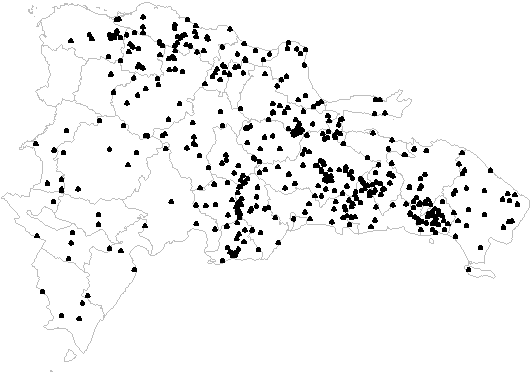
\includegraphics{proyecto_files/figure-latex/unnamed-chunk-6-1.pdf}

\subsection{Estadísticos básicos para la capa de
sismos}\label{estaduxedsticos-buxe1sicos-para-la-capa-de-sismos}

\begin{Shaded}
\begin{Highlighting}[]
\KeywordTok{nrow}\NormalTok{(sismos)}
\end{Highlighting}
\end{Shaded}

\begin{verbatim}
## [1] 439
\end{verbatim}

\begin{Shaded}
\begin{Highlighting}[]
\KeywordTok{summary}\NormalTok{(sismos}\OperatorTok{$}\NormalTok{MAGNITUD)}
\end{Highlighting}
\end{Shaded}

\begin{verbatim}
##    Min. 1st Qu.  Median    Mean 3rd Qu.    Max. 
##   1.670   2.820   3.070   3.053   3.275   4.430
\end{verbatim}

\begin{Shaded}
\begin{Highlighting}[]
\KeywordTok{hist}\NormalTok{(sismos}\OperatorTok{$}\NormalTok{MAGNITUD)}
\end{Highlighting}
\end{Shaded}

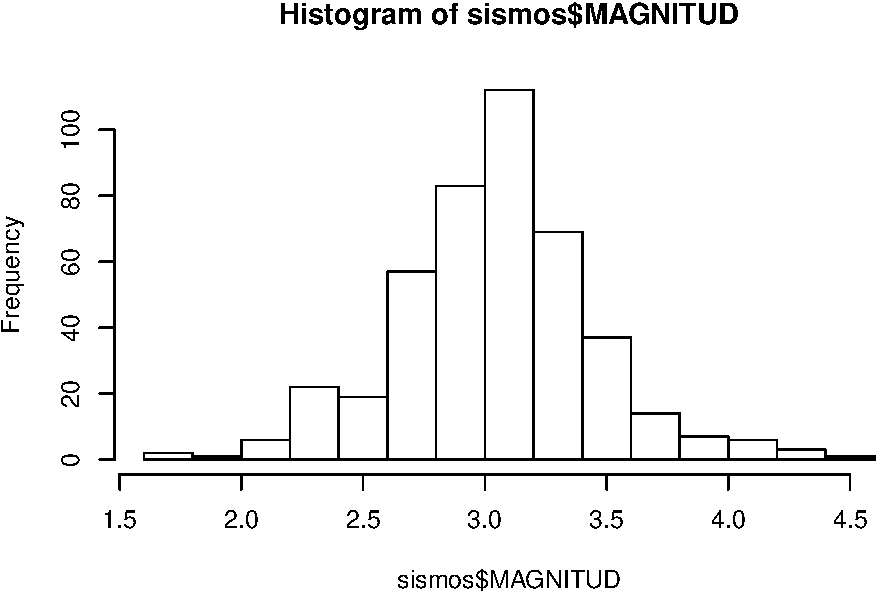
\includegraphics{proyecto_files/figure-latex/unnamed-chunk-7-1.pdf}

\begin{Shaded}
\begin{Highlighting}[]
\KeywordTok{hist}\NormalTok{(}\KeywordTok{log}\NormalTok{(sismos}\OperatorTok{$}\NormalTok{MAGNITUD))}
\end{Highlighting}
\end{Shaded}

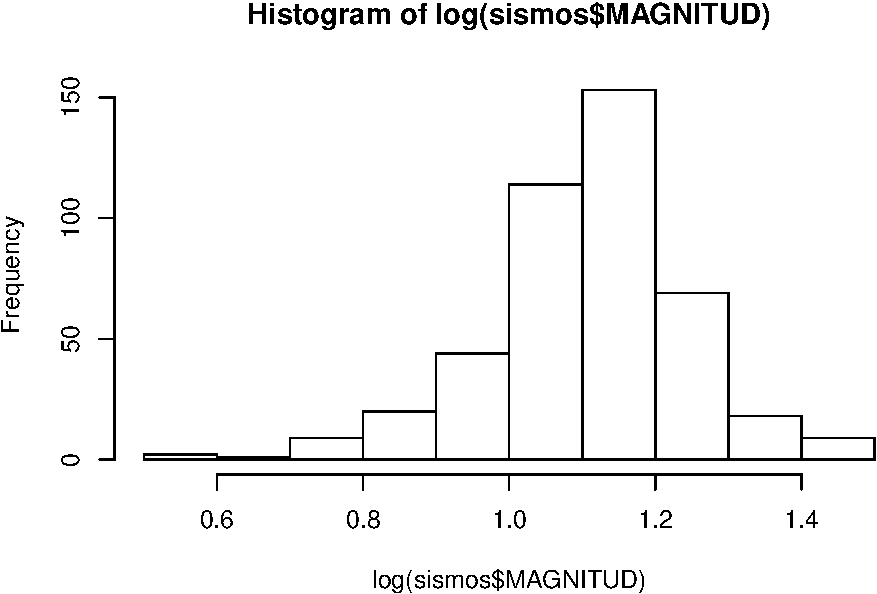
\includegraphics{proyecto_files/figure-latex/unnamed-chunk-7-2.pdf}

\begin{Shaded}
\begin{Highlighting}[]
\KeywordTok{shapiro.test}\NormalTok{(sismos}\OperatorTok{$}\NormalTok{MAGNITUD)}
\end{Highlighting}
\end{Shaded}

\begin{verbatim}
## 
##  Shapiro-Wilk normality test
## 
## data:  sismos$MAGNITUD
## W = 0.98381, p-value = 8.151e-05
\end{verbatim}

\begin{Shaded}
\begin{Highlighting}[]
\KeywordTok{shapiro.test}\NormalTok{(}\KeywordTok{log}\NormalTok{(sismos}\OperatorTok{$}\NormalTok{MAGNITUD))}
\end{Highlighting}
\end{Shaded}

\begin{verbatim}
## 
##  Shapiro-Wilk normality test
## 
## data:  log(sismos$MAGNITUD)
## W = 0.97136, p-value = 1.419e-07
\end{verbatim}

\begin{Shaded}
\begin{Highlighting}[]
\KeywordTok{qqnorm}\NormalTok{(sismos}\OperatorTok{$}\NormalTok{MAGNITUD)}
\end{Highlighting}
\end{Shaded}

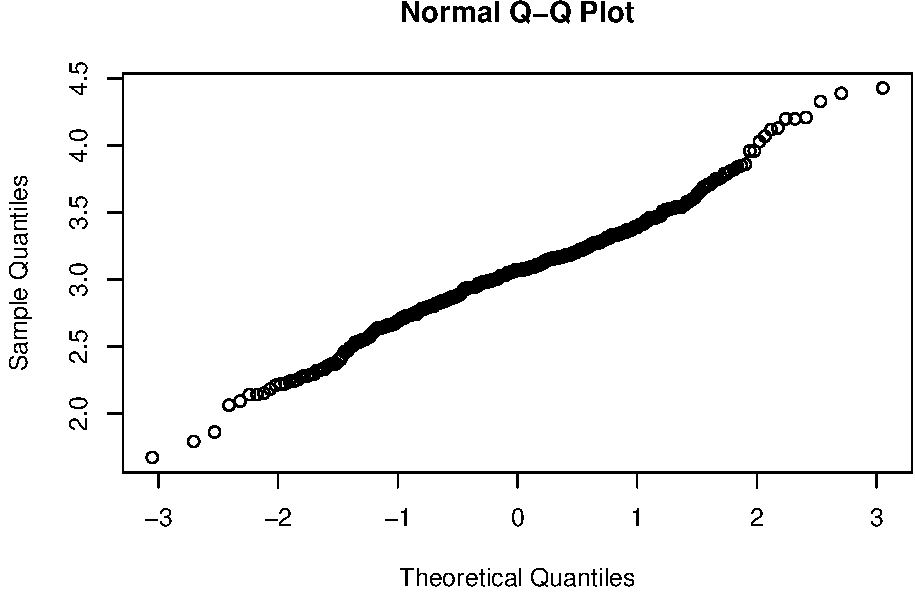
\includegraphics{proyecto_files/figure-latex/unnamed-chunk-7-3.pdf}

\begin{Shaded}
\begin{Highlighting}[]
\KeywordTok{qqnorm}\NormalTok{(}\KeywordTok{log}\NormalTok{(sismos}\OperatorTok{$}\NormalTok{MAGNITUD))}
\end{Highlighting}
\end{Shaded}

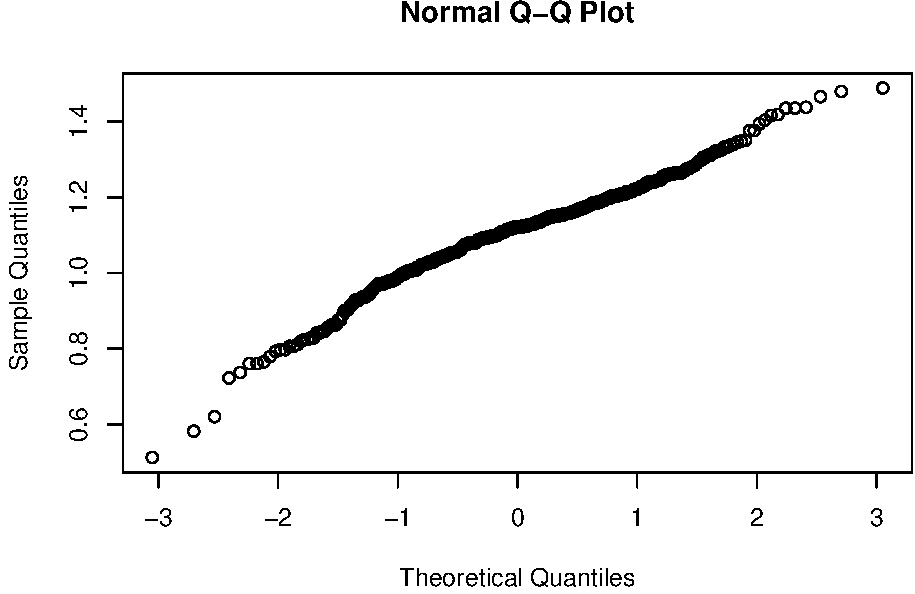
\includegraphics{proyecto_files/figure-latex/unnamed-chunk-7-4.pdf}

\begin{Shaded}
\begin{Highlighting}[]
\KeywordTok{boxplot}\NormalTok{(sismos}\OperatorTok{$}\NormalTok{MAGNITUD)}
\end{Highlighting}
\end{Shaded}

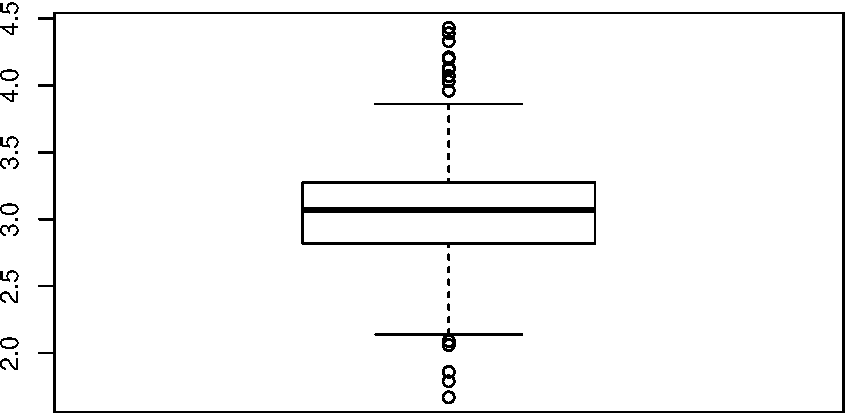
\includegraphics{proyecto_files/figure-latex/unnamed-chunk-7-5.pdf}

\subsubsection{Generacion de variograma para la capa de
sismos}\label{generacion-de-variograma-para-la-capa-de-sismos}

\begin{Shaded}
\begin{Highlighting}[]
\NormalTok{vsismos <-}\StringTok{ }\KeywordTok{variogram}\NormalTok{(MAGNITUD}\OperatorTok{~}\DecValTok{1}\NormalTok{, sismos)}
\KeywordTok{plot}\NormalTok{(vsismos)}
\end{Highlighting}
\end{Shaded}

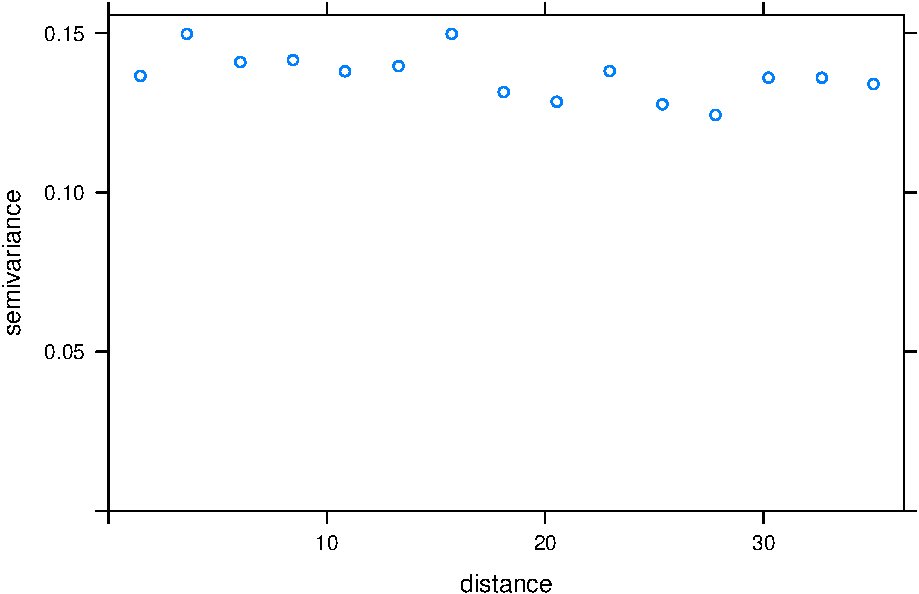
\includegraphics{proyecto_files/figure-latex/unnamed-chunk-8-1.pdf}

\subsubsection{Despliege de estadisticos de la magnitud de los sismos y
graficado de estos en la capa de
provincias}\label{despliege-de-estadisticos-de-la-magnitud-de-los-sismos-y-graficado-de-estos-en-la-capa-de-provincias}

\begin{Shaded}
\begin{Highlighting}[]
\NormalTok{sismosprovdf <-}\StringTok{ }\NormalTok{prov }\OperatorTok
\StringTok{  }\KeywordTok{st_intersection}\NormalTok{(sismosutm) }\OperatorTok
\StringTok{  }\KeywordTok{st_drop_geometry}\NormalTok{() }\OperatorTok
\StringTok{  }\KeywordTok{select}\NormalTok{(ENLACE, MAGNITUD) }\OperatorTok
\StringTok{  }\KeywordTok{group_by}\NormalTok{(ENLACE) }\OperatorTok
\StringTok{  }\KeywordTok{summarise}\NormalTok{(}\DataTypeTok{med=}\KeywordTok{mean}\NormalTok{(MAGNITUD, }\DataTypeTok{na.rm=}\NormalTok{T), }\DataTypeTok{var=}\KeywordTok{var}\NormalTok{(MAGNITUD, }\DataTypeTok{na.rm =}\NormalTok{ T),}
            \DataTypeTok{min=}\KeywordTok{min}\NormalTok{(MAGNITUD, }\DataTypeTok{na.rm=}\NormalTok{T), }\DataTypeTok{max=}\KeywordTok{max}\NormalTok{(MAGNITUD, }\DataTypeTok{na.rm =}\NormalTok{ T), }\DataTypeTok{N=}\KeywordTok{n}\NormalTok{())}
\end{Highlighting}
\end{Shaded}

\begin{verbatim}
## Warning: attribute variables are assumed to be spatially constant
## throughout all geometries
\end{verbatim}

\begin{Shaded}
\begin{Highlighting}[]
\NormalTok{sismosprovsf <-}\StringTok{ }\NormalTok{prov }\OperatorTok\StringTok{ }\KeywordTok{inner_join}\NormalTok{(sismosprovdf, }\DataTypeTok{by =} \StringTok{'ENLACE'}\NormalTok{)}
\NormalTok{sismosprovsf}
\end{Highlighting}
\end{Shaded}

\begin{verbatim}
## Simple feature collection with 31 features and 9 fields
## geometry type:  MULTIPOLYGON
## dimension:      XY
## bbox:           xmin: 182215.8 ymin: 1933532 xmax: 571365.3 ymax: 2205216
## epsg (SRID):    32619
## proj4string:    +proj=utm +zone=19 +datum=WGS84 +units=m +no_defs
## First 10 features:
##    PROV REG         TOPONIMIA ENLACE      med       var  min  max  N
## 1    01  10 DISTRITO NACIONAL   1001 2.730000        NA 2.73 2.73  1
## 2    02  05              AZUA   0502 2.948000 0.0658200 2.61 3.23  5
## 3    03  06           BAORUCO   0603 2.450000 0.2592000 2.09 2.81  2
## 4    04  06          BARAHONA   0604 2.743333 0.2410333 2.18 3.08  3
## 5    06  03            DUARTE   0306 2.841111 0.2434105 1.67 3.37 18
## 6    07  07        ELÍAS PIÑA   0707 2.647143 0.1162571 2.32 3.18  7
## 7    08  08          EL SEIBO   0808 3.275789 0.1907702 2.55 4.13 19
## 8    09  01         ESPAILLAT   0109 3.200667 0.1527924 2.73 4.43 15
## 9    10  06     INDEPENDENCIA   0610 2.740000 0.2671200 2.24 3.53  6
## 10   11  08     LA ALTAGRACIA   0811 3.461667 0.1093014 2.82 4.39 24
##                              geom
## 1  MULTIPOLYGON (((406845.9 20...
## 2  MULTIPOLYGON (((322129.5 20...
## 3  MULTIPOLYGON (((271940 2060...
## 4  MULTIPOLYGON (((291856.5 20...
## 5  MULTIPOLYGON (((374434.8 21...
## 6  MULTIPOLYGON (((235630.8 21...
## 7  MULTIPOLYGON (((523436.4 20...
## 8  MULTIPOLYGON (((385993.5 21...
## 9  MULTIPOLYGON (((205698.2 20...
## 10 MULTIPOLYGON (((516555.9 20...
\end{verbatim}

\begin{Shaded}
\begin{Highlighting}[]
\KeywordTok{plot}\NormalTok{(sismosprovsf)}
\end{Highlighting}
\end{Shaded}

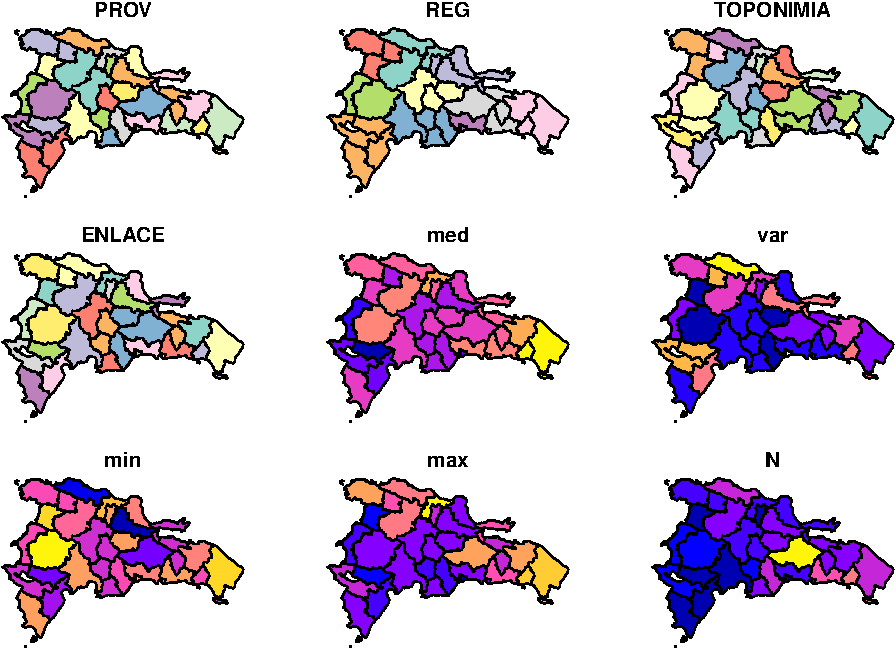
\includegraphics{proyecto_files/figure-latex/unnamed-chunk-9-1.pdf}

\subsection{Vecindad}\label{vecindad}

\begin{Shaded}
\begin{Highlighting}[]
\KeywordTok{rownames}\NormalTok{(sismosprovsf) <-}\StringTok{ }\NormalTok{sismosprovsf}\OperatorTok{$}\NormalTok{TOPONIMIA}
\NormalTok{nb <-}\StringTok{ }\KeywordTok{poly2nb}\NormalTok{(sismosprovsf)}
\KeywordTok{summary}\NormalTok{(nb)}
\end{Highlighting}
\end{Shaded}

\begin{verbatim}
## Neighbour list object:
## Number of regions: 31 
## Number of nonzero links: 138 
## Percentage nonzero weights: 14.36004 
## Average number of links: 4.451613 
## Link number distribution:
## 
## 1 2 3 4 5 6 7 8 9 
## 1 2 6 9 6 3 2 1 1 
## 1 least connected region:
## DISTRITO NACIONAL with 1 link
## 1 most connected region:
## LA VEGA with 9 links
\end{verbatim}

\begin{Shaded}
\begin{Highlighting}[]
\KeywordTok{is.symmetric.nb}\NormalTok{(nb)}
\end{Highlighting}
\end{Shaded}

\begin{verbatim}
## [1] TRUE
\end{verbatim}

\begin{Shaded}
\begin{Highlighting}[]
\KeywordTok{card}\NormalTok{(nb)}
\end{Highlighting}
\end{Shaded}

\begin{verbatim}
##  [1] 1 6 4 4 7 3 4 6 5 2 3 9 3 3 2 3 4 3 4 5 7 5 4 6 5 4 5 8 4 5 4
\end{verbatim}

\subsubsection{Ponderadores espaciales (Pesos), estandarizado por filas
(w.W) y binario
(w.B)}\label{ponderadores-espaciales-pesos-estandarizado-por-filas-w.w-y-binario-w.b}

\begin{Shaded}
\begin{Highlighting}[]
\NormalTok{wW <-}\StringTok{ }\KeywordTok{nb2listw}\NormalTok{(nb)}
\KeywordTok{summary}\NormalTok{(wW)}
\end{Highlighting}
\end{Shaded}

\begin{verbatim}
## Characteristics of weights list object:
## Neighbour list object:
## Number of regions: 31 
## Number of nonzero links: 138 
## Percentage nonzero weights: 14.36004 
## Average number of links: 4.451613 
## Link number distribution:
## 
## 1 2 3 4 5 6 7 8 9 
## 1 2 6 9 6 3 2 1 1 
## 1 least connected region:
## DISTRITO NACIONAL with 1 link
## 1 most connected region:
## LA VEGA with 9 links
## 
## Weights style: W 
## Weights constants summary:
##    n  nn S0       S1       S2
## W 31 961 31 15.53669 128.9319
\end{verbatim}

\begin{Shaded}
\begin{Highlighting}[]
\NormalTok{wB <-}\StringTok{ }\KeywordTok{nb2listw}\NormalTok{(nb, }\DataTypeTok{style =} \StringTok{'B'}\NormalTok{)}
\KeywordTok{summary}\NormalTok{(wB)}
\end{Highlighting}
\end{Shaded}

\begin{verbatim}
## Characteristics of weights list object:
## Neighbour list object:
## Number of regions: 31 
## Number of nonzero links: 138 
## Percentage nonzero weights: 14.36004 
## Average number of links: 4.451613 
## Link number distribution:
## 
## 1 2 3 4 5 6 7 8 9 
## 1 2 6 9 6 3 2 1 1 
## 1 least connected region:
## DISTRITO NACIONAL with 1 link
## 1 most connected region:
## LA VEGA with 9 links
## 
## Weights style: B 
## Weights constants summary:
##    n  nn  S0  S1   S2
## B 31 961 138 276 2832
\end{verbatim}

\subsubsection{Prueba de Breusch-Pagan}\label{prueba-de-breusch-pagan-1}

Se preparan los datos y se añaden columnas x,y

\begin{Shaded}
\begin{Highlighting}[]
\NormalTok{coordsxy <-}\StringTok{ }\NormalTok{sismosprovsf }\OperatorTok
\StringTok{  }\KeywordTok{st_centroid}\NormalTok{() }\OperatorTok\StringTok{ }
\StringTok{  }\KeywordTok{mutate}\NormalTok{(}\DataTypeTok{x=}\KeywordTok{unlist}\NormalTok{(}\KeywordTok{map}\NormalTok{(geom,}\DecValTok{1}\NormalTok{)),}
         \DataTypeTok{y=}\KeywordTok{unlist}\NormalTok{(}\KeywordTok{map}\NormalTok{(geom,}\DecValTok{2}\NormalTok{))) }\OperatorTok
\StringTok{  }\KeywordTok{st_drop_geometry}\NormalTok{() }\OperatorTok\StringTok{ }
\StringTok{  }\KeywordTok{select}\NormalTok{(ENLACE, x, y)}
\end{Highlighting}
\end{Shaded}

\begin{verbatim}
## Warning in st_centroid.sf(.): st_centroid assumes attributes are constant
## over geometries of x
\end{verbatim}

\begin{Shaded}
\begin{Highlighting}[]
\NormalTok{coordsxy}
\end{Highlighting}
\end{Shaded}

\begin{verbatim}
##    ENLACE        x       y
## 1    1001 400578.3 2044093
## 2    0502 306538.2 2055500
## 3    0603 253648.9 2048423
## 4    0604 265654.1 2010069
## 5    0306 386306.5 2129851
## 6    0707 225124.2 2102815
## 7    0808 495201.2 2080870
## 8    0109 353886.4 2160683
## 9    0610 223355.0 2038578
## 10   0811 536305.4 2054312
## 11   0812 507981.8 2039462
## 12   0213 328347.6 2107572
## 13   0314 398288.3 2150595
## 14   0415 243239.8 2182499
## 15   0616 231492.7 1986919
## 16   0517 354976.3 2027668
## 17   0118 311509.7 2184236
## 18   0319 356316.3 2147557
## 19   0320 449157.4 2125956
## 20   0521 372616.4 2048411
## 21   0722 258835.2 2088747
## 22   0923 461906.6 2051259
## 23   0224 380195.2 2103276
## 24   0125 300355.2 2138416
## 25   0426 255988.3 2144472
## 26   0427 285842.4 2166909
## 27   0228 350949.4 2091009
## 28   0929 415757.1 2082988
## 29   0930 461031.9 2085855
## 30   0531 342264.4 2059304
## 31   1032 410362.0 2053166
\end{verbatim}

\begin{Shaded}
\begin{Highlighting}[]
\NormalTok{sismosprovsf <-}\StringTok{ }\NormalTok{sismosprovsf }\OperatorTok
\StringTok{  }\KeywordTok{inner_join}\NormalTok{(coordsxy)}
\end{Highlighting}
\end{Shaded}

\begin{verbatim}
## Joining, by = "ENLACE"
\end{verbatim}

\begin{Shaded}
\begin{Highlighting}[]
\NormalTok{sismosprovsf }\OperatorTok\StringTok{ }\KeywordTok{lm}\NormalTok{(med}\OperatorTok{~}\StringTok{ }\NormalTok{x, .) }\OperatorTok\StringTok{ }\KeywordTok{plot}\NormalTok{(}\DecValTok{3}\NormalTok{)}
\end{Highlighting}
\end{Shaded}

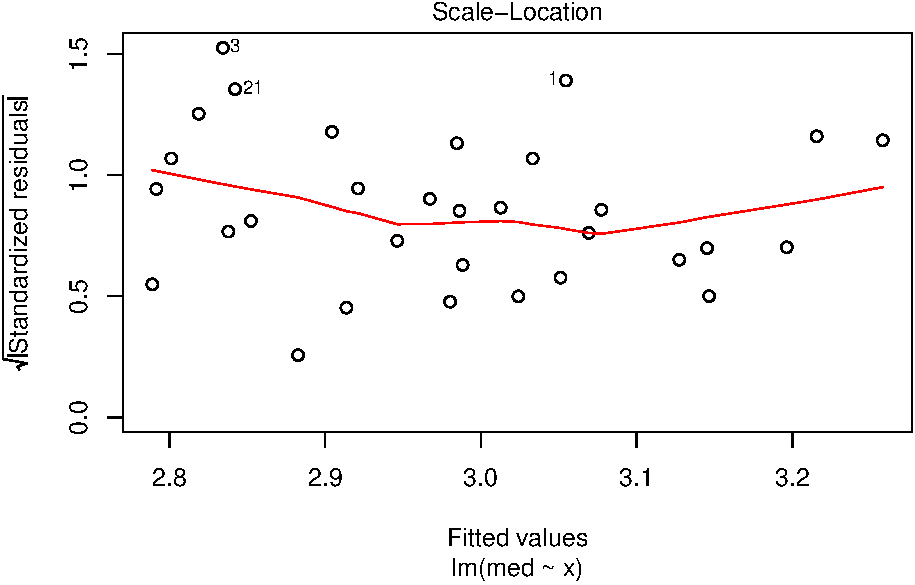
\includegraphics{proyecto_files/figure-latex/unnamed-chunk-12-1.pdf}

\begin{Shaded}
\begin{Highlighting}[]
\NormalTok{sismosprovsf }\OperatorTok\StringTok{ }\KeywordTok{lm}\NormalTok{(med}\OperatorTok{~}\StringTok{ }\NormalTok{y, .) }\OperatorTok\StringTok{ }\KeywordTok{plot}\NormalTok{(}\DecValTok{3}\NormalTok{)}
\end{Highlighting}
\end{Shaded}

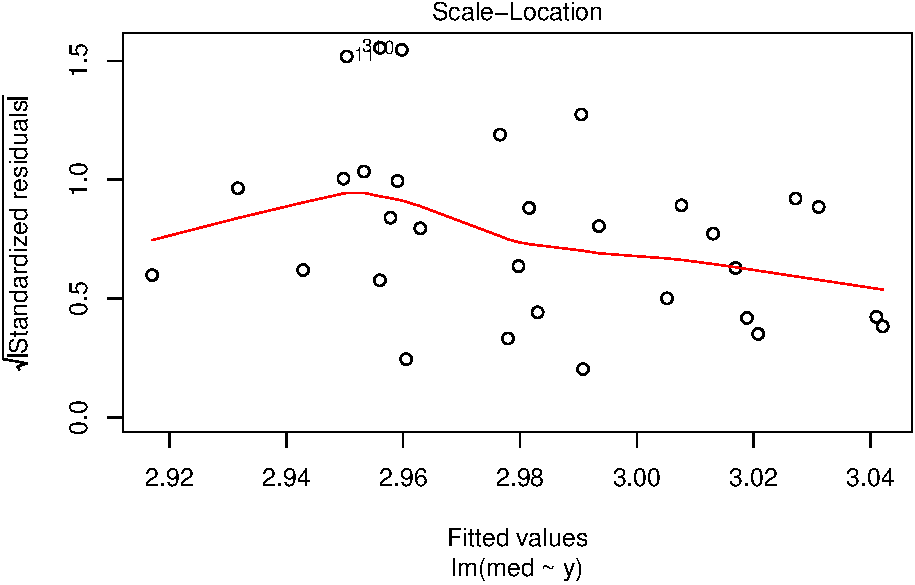
\includegraphics{proyecto_files/figure-latex/unnamed-chunk-12-2.pdf}

\begin{Shaded}
\begin{Highlighting}[]
\NormalTok{sismosprovsf }\OperatorTok\StringTok{ }\KeywordTok{lm}\NormalTok{(med}\OperatorTok{~}\StringTok{ }\NormalTok{x, .) }\OperatorTok\StringTok{ }\KeywordTok{bptest}\NormalTok{()}
\end{Highlighting}
\end{Shaded}

\begin{verbatim}
## 
##  studentized Breusch-Pagan test
## 
## data:  .
## BP = 1.2218, df = 1, p-value = 0.269
\end{verbatim}

\begin{Shaded}
\begin{Highlighting}[]
\NormalTok{sismosprovsf }\OperatorTok\StringTok{ }\KeywordTok{lm}\NormalTok{(med}\OperatorTok{~}\StringTok{ }\NormalTok{y, .) }\OperatorTok\StringTok{ }\KeywordTok{bptest}\NormalTok{()}
\end{Highlighting}
\end{Shaded}

\begin{verbatim}
## 
##  studentized Breusch-Pagan test
## 
## data:  .
## BP = 2.9431, df = 1, p-value = 0.08624
\end{verbatim}

\subsubsection{Autocorrelación global por I de
Moran}\label{autocorrelaciuxf3n-global-por-i-de-moran-1}

\begin{Shaded}
\begin{Highlighting}[]
\NormalTok{(gmoranw <-}\StringTok{ }\KeywordTok{moran.test}\NormalTok{(}\DataTypeTok{x =}\NormalTok{ sismosprovsf}\OperatorTok{$}\NormalTok{med, }\DataTypeTok{listw =}\NormalTok{ wW, }\DataTypeTok{na.action =}\NormalTok{ na.omit))}
\end{Highlighting}
\end{Shaded}

\begin{verbatim}
## 
##  Moran I test under randomisation
## 
## data:  sismosprovsf$med  
## weights: wW    
## 
## Moran I statistic standard deviate = 3.5838, p-value = 0.0001693
## alternative hypothesis: greater
## sample estimates:
## Moran I statistic       Expectation          Variance 
##        0.38347105       -0.03333333        0.01352607
\end{verbatim}

\begin{Shaded}
\begin{Highlighting}[]
\NormalTok{(gmoranb <-}\StringTok{ }\KeywordTok{moran.test}\NormalTok{(}\DataTypeTok{x =}\NormalTok{ sismosprovsf}\OperatorTok{$}\NormalTok{med, }\DataTypeTok{listw =}\NormalTok{ wB, }\DataTypeTok{na.action =}\NormalTok{ na.omit))}
\end{Highlighting}
\end{Shaded}

\begin{verbatim}
## 
##  Moran I test under randomisation
## 
## data:  sismosprovsf$med  
## weights: wB    
## 
## Moran I statistic standard deviate = 2.9675, p-value = 0.001501
## alternative hypothesis: greater
## sample estimates:
## Moran I statistic       Expectation          Variance 
##        0.28414338       -0.03333333        0.01144585
\end{verbatim}

\subsubsection{Autocorrelación local por
magnitud}\label{autocorrelaciuxf3n-local-por-magnitud-1}

\begin{Shaded}
\begin{Highlighting}[]
\KeywordTok{moran.plot}\NormalTok{(}\DataTypeTok{x =}\NormalTok{ sismosprovsf}\OperatorTok{$}\NormalTok{med, }\DataTypeTok{listw =}\NormalTok{ wW)}
\end{Highlighting}
\end{Shaded}

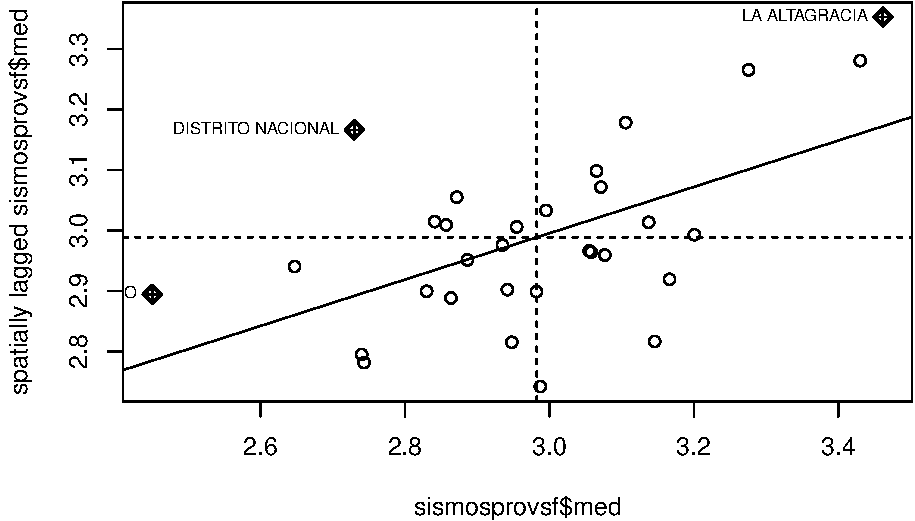
\includegraphics{proyecto_files/figure-latex/unnamed-chunk-14-1.pdf}

\begin{Shaded}
\begin{Highlighting}[]
\KeywordTok{source}\NormalTok{(}\StringTok{'lisaclusters.R'}\NormalTok{)}
\KeywordTok{lisamap}\NormalTok{(}\DataTypeTok{objesp =}\NormalTok{  sismosprovsf,}
        \DataTypeTok{var =} \StringTok{'med'}\NormalTok{,}
        \DataTypeTok{pesos =}\NormalTok{ wW,}
        \DataTypeTok{tituloleyenda =} \StringTok{'Significancia}\CharTok{\textbackslash{}n}\StringTok{("x-y", léase}\CharTok{\textbackslash{}n}\StringTok{como "x"}\CharTok{\textbackslash{}n}\StringTok{rodeado de "y"'}\NormalTok{,}
        \DataTypeTok{leyenda =}\NormalTok{ T,}
        \DataTypeTok{anchuratitulo =} \DecValTok{1000}\NormalTok{,}
        \DataTypeTok{tamanotitulo =} \DecValTok{16}\NormalTok{,}
        \DataTypeTok{fuentedatos =} \StringTok{'CNS'}\NormalTok{,}
        \DataTypeTok{titulomapa =} \KeywordTok{paste0}\NormalTok{(}\StringTok{'Clusters LISA de media de la magnitud de sismos de 2014'}\NormalTok{))}
\end{Highlighting}
\end{Shaded}

\begin{verbatim}
## $grafico
\end{verbatim}

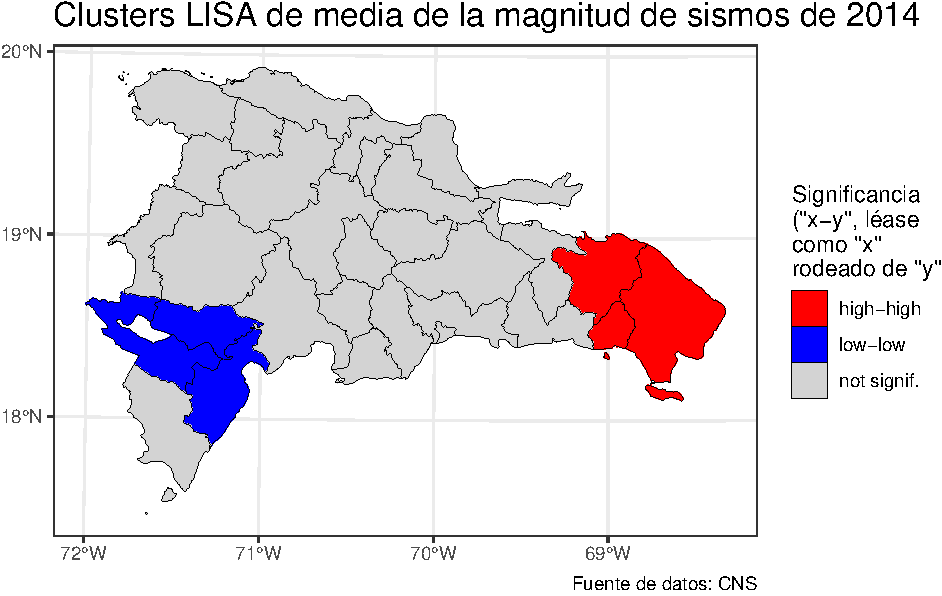
\includegraphics{proyecto_files/figure-latex/unnamed-chunk-14-2.pdf}

\begin{verbatim}
## 
## $objeto
## Simple feature collection with 31 features and 14 fields
## geometry type:  MULTIPOLYGON
## dimension:      XY
## bbox:           xmin: 182215.8 ymin: 1933532 xmax: 571365.3 ymax: 2205216
## epsg (SRID):    32619
## proj4string:    +proj=utm +zone=19 +datum=WGS84 +units=m +no_defs
## First 10 features:
##    PROV REG         TOPONIMIA ENLACE      med       var  min  max  N
## 1    01  10 DISTRITO NACIONAL   1001 2.730000        NA 2.73 2.73  1
## 2    02  05              AZUA   0502 2.948000 0.0658200 2.61 3.23  5
## 3    03  06           BAORUCO   0603 2.450000 0.2592000 2.09 2.81  2
## 4    04  06          BARAHONA   0604 2.743333 0.2410333 2.18 3.08  3
## 5    06  03            DUARTE   0306 2.841111 0.2434105 1.67 3.37 18
## 6    07  07        ELÍAS PIÑA   0707 2.647143 0.1162571 2.32 3.18  7
## 7    08  08          EL SEIBO   0808 3.275789 0.1907702 2.55 4.13 19
## 8    09  01         ESPAILLAT   0109 3.200667 0.1527924 2.73 4.43 15
## 9    10  06     INDEPENDENCIA   0610 2.740000 0.2671200 2.24 3.53  6
## 10   11  08     LA ALTAGRACIA   0811 3.461667 0.1093014 2.82 4.39 24
##           x       y                           geom puntuacionz
## 1  400578.3 2044093 MULTIPOLYGON (((406845.9 20...  -1.1792229
## 2  306538.2 2055500 MULTIPOLYGON (((322129.5 20...  -0.1607081
## 3  253648.9 2048423 MULTIPOLYGON (((271940 2060...  -2.4874069
## 4  265654.1 2010069 MULTIPOLYGON (((291856.5 20...  -1.1169284
## 5  386306.5 2129851 MULTIPOLYGON (((374434.8 21...  -0.6601022
## 6  225124.2 2102815 MULTIPOLYGON (((235630.8 21...  -1.5663386
## 7  495201.2 2080870 MULTIPOLYGON (((523436.4 20...   1.3707524
## 8  353886.4 2160683 MULTIPOLYGON (((385993.5 21...   1.0197722
## 9  223355.0 2038578 MULTIPOLYGON (((205698.2 20...  -1.1325020
## 10 536305.4 2054312 MULTIPOLYGON (((516555.9 20...   2.2391867
##    lagpuntuacionz    quad_sig
## 1      0.85950554 not signif.
## 2     -0.78236428 not signif.
## 3     -0.41177713     low-low
## 4     -0.93919445     low-low
## 5      0.15062150 not signif.
## 6     -0.19697242 not signif.
## 7      1.32362286   high-high
## 8      0.04888849 not signif.
## 9     -0.87676092     low-low
## 10     1.73174843   high-high
\end{verbatim}

\subsubsection{Autocorrelación local por cantidad de
eventos}\label{autocorrelaciuxf3n-local-por-cantidad-de-eventos-1}

\begin{Shaded}
\begin{Highlighting}[]
\KeywordTok{moran.plot}\NormalTok{(}\DataTypeTok{x =}\NormalTok{ sismosprovsf}\OperatorTok{$}\NormalTok{N, }\DataTypeTok{listw =}\NormalTok{ wW)}
\end{Highlighting}
\end{Shaded}

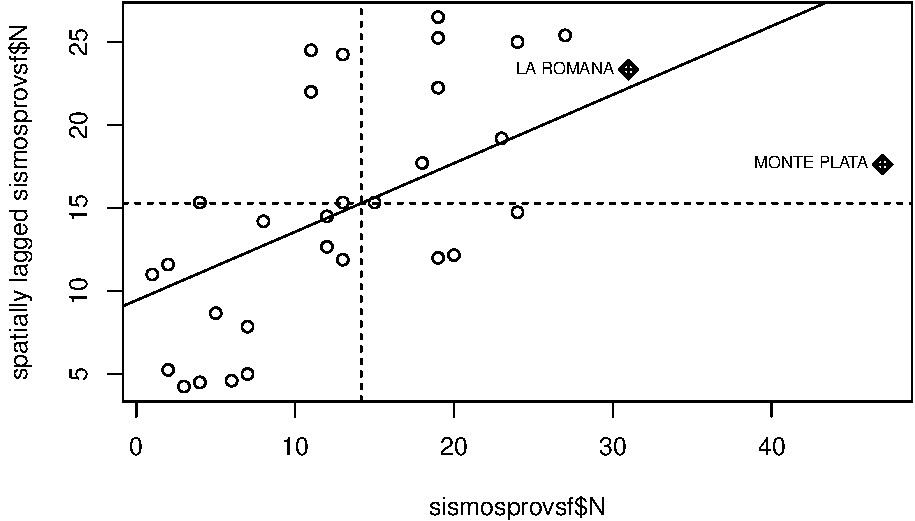
\includegraphics{proyecto_files/figure-latex/unnamed-chunk-15-1.pdf}

\begin{Shaded}
\begin{Highlighting}[]
\KeywordTok{lisamap}\NormalTok{(}\DataTypeTok{objesp =}\NormalTok{  sismosprovsf,}
        \DataTypeTok{var =} \StringTok{'N'}\NormalTok{,}
        \DataTypeTok{pesos =}\NormalTok{ wW,}
        \DataTypeTok{tituloleyenda =} \StringTok{'Significancia}\CharTok{\textbackslash{}n}\StringTok{("x-y", léase}\CharTok{\textbackslash{}n}\StringTok{como "x"}\CharTok{\textbackslash{}n}\StringTok{rodeado de "y"'}\NormalTok{,}
        \DataTypeTok{leyenda =}\NormalTok{ T,}
        \DataTypeTok{anchuratitulo =} \DecValTok{1000}\NormalTok{,}
        \DataTypeTok{tamanotitulo =} \DecValTok{16}\NormalTok{,}
        \DataTypeTok{fuentedatos =} \StringTok{'CNS'}\NormalTok{,}
        \DataTypeTok{titulomapa =} \KeywordTok{paste0}\NormalTok{(}\StringTok{'Clusters LISA del número de sismos de 2014'}\NormalTok{))}
\end{Highlighting}
\end{Shaded}

\begin{verbatim}
## $grafico
\end{verbatim}

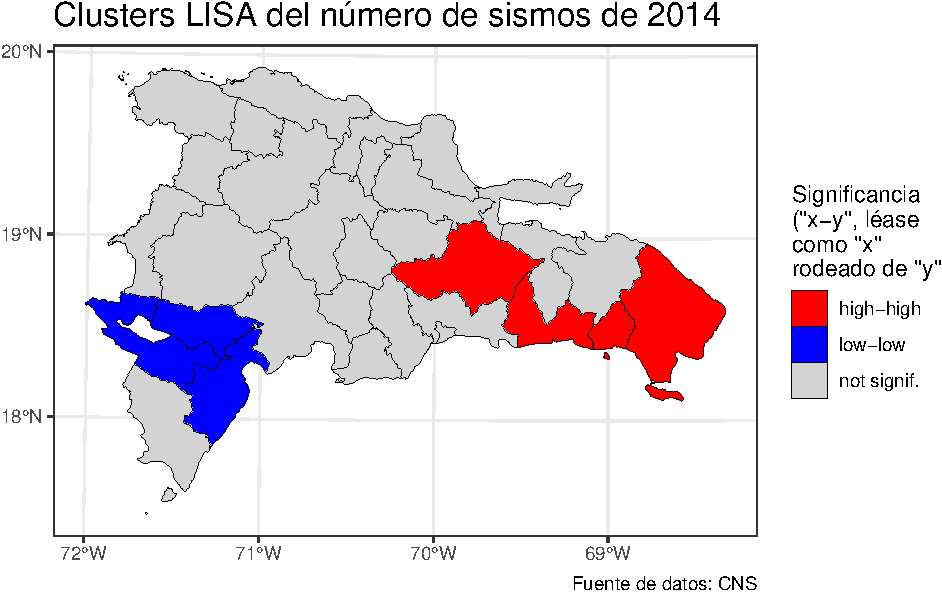
\includegraphics{proyecto_files/figure-latex/unnamed-chunk-15-2.pdf}

\begin{verbatim}
## 
## $objeto
## Simple feature collection with 31 features and 14 fields
## geometry type:  MULTIPOLYGON
## dimension:      XY
## bbox:           xmin: 182215.8 ymin: 1933532 xmax: 571365.3 ymax: 2205216
## epsg (SRID):    32619
## proj4string:    +proj=utm +zone=19 +datum=WGS84 +units=m +no_defs
## First 10 features:
##    PROV REG         TOPONIMIA ENLACE      med       var  min  max  N
## 1    01  10 DISTRITO NACIONAL   1001 2.730000        NA 2.73 2.73  1
## 2    02  05              AZUA   0502 2.948000 0.0658200 2.61 3.23  5
## 3    03  06           BAORUCO   0603 2.450000 0.2592000 2.09 2.81  2
## 4    04  06          BARAHONA   0604 2.743333 0.2410333 2.18 3.08  3
## 5    06  03            DUARTE   0306 2.841111 0.2434105 1.67 3.37 18
## 6    07  07        ELÍAS PIÑA   0707 2.647143 0.1162571 2.32 3.18  7
## 7    08  08          EL SEIBO   0808 3.275789 0.1907702 2.55 4.13 19
## 8    09  01         ESPAILLAT   0109 3.200667 0.1527924 2.73 4.43 15
## 9    10  06     INDEPENDENCIA   0610 2.740000 0.2671200 2.24 3.53  6
## 10   11  08     LA ALTAGRACIA   0811 3.461667 0.1093014 2.82 4.39 24
##           x       y                           geom puntuacionz
## 1  400578.3 2044093 MULTIPOLYGON (((406845.9 20... -1.30184510
## 2  306538.2 2055500 MULTIPOLYGON (((322129.5 20... -0.90618630
## 3  253648.9 2048423 MULTIPOLYGON (((271940 2060... -1.20293040
## 4  265654.1 2010069 MULTIPOLYGON (((291856.5 20... -1.10401570
## 5  386306.5 2129851 MULTIPOLYGON (((374434.8 21...  0.37970482
## 6  225124.2 2102815 MULTIPOLYGON (((235630.8 21... -0.70835689
## 7  495201.2 2080870 MULTIPOLYGON (((523436.4 20...  0.47861952
## 8  353886.4 2160683 MULTIPOLYGON (((385993.5 21...  0.08296072
## 9  223355.0 2038578 MULTIPOLYGON (((205698.2 20... -0.80727160
## 10 536305.4 2054312 MULTIPOLYGON (((516555.9 20...  0.97319303
##    lagpuntuacionz    quad_sig
## 1      -0.3126981 not signif.
## 2      -0.5434991 not signif.
## 3      -0.8814576     low-low
## 4      -0.9803723     low-low
## 5       0.3514435 not signif.
## 6      -0.9061863 not signif.
## 7       1.0968364 not signif.
## 8       0.1159323 not signif.
## 9      -0.9457522     low-low
## 10      1.0721077   high-high
\end{verbatim}

\subsection{Estadística zonal}\label{estaduxedstica-zonal-1}

\begin{Shaded}
\begin{Highlighting}[]
\NormalTok{devtools}\OperatorTok{::}\KeywordTok{source_url}\NormalTok{(}\StringTok{'https://raw.githubusercontent.com/geofis/zonal-stats-sf/master/zonal-stats-sf.R'}\NormalTok{)}
\end{Highlighting}
\end{Shaded}

\begin{verbatim}
## SHA-1 hash of file is 39a34cd2f8ac93e5f6d576a9da514ec44950c4db
\end{verbatim}

\begin{Shaded}
\begin{Highlighting}[]
\NormalTok{ezfallasprov <-}\StringTok{ }\KeywordTok{zstatsf}\NormalTok{(}\DataTypeTok{zones =}\NormalTok{ prov, }\DataTypeTok{values =}\NormalTok{ fallasmayores, }\DataTypeTok{grpx =} \StringTok{'TOPONIMIA'}\NormalTok{, }\DataTypeTok{grpy =} \StringTok{'TIPOGLOBAL'}\NormalTok{)}
\end{Highlighting}
\end{Shaded}

Uniendo con el \texttt{sf} central:

\begin{Shaded}
\begin{Highlighting}[]
\NormalTok{sismosprovsf2 <-}\StringTok{ }\NormalTok{sismosprovsf }\OperatorTok
\StringTok{  }\KeywordTok{right_join}\NormalTok{(ezfallasprov }\OperatorTok\StringTok{ }\NormalTok{st_drop_geometry }\OperatorTok\StringTok{ }\KeywordTok{rename}\NormalTok{(}\DataTypeTok{km_falla_por_km2 =} \StringTok{`}\DataTypeTok{falla indiferenciado}\StringTok{`}\NormalTok{), }\DataTypeTok{by =} \StringTok{'TOPONIMIA'}\NormalTok{)}
\end{Highlighting}
\end{Shaded}

Densidad de fallas geológicas por provincias

\begin{Shaded}
\begin{Highlighting}[]
\NormalTok{sismosprovsf2 }\OperatorTok\StringTok{ }\KeywordTok{st_drop_geometry}\NormalTok{() }\OperatorTok
\StringTok{  }\NormalTok{dplyr}\OperatorTok{::}\KeywordTok{select}\NormalTok{(TOPONIMIA,km_falla_por_km2)}
\end{Highlighting}
\end{Shaded}

\begin{verbatim}
##                 TOPONIMIA km_falla_por_km2
## 1                    AZUA       149.705774
## 2                 BAORUCO        90.429174
## 3                BARAHONA       148.071735
## 4                 DAJABÓN        33.435485
## 5                  DUARTE       156.167525
## 6                EL SEIBO        68.751545
## 7              ELÍAS PIÑA       103.615453
## 8               ESPAILLAT       182.850996
## 9              HATO MAYOR        47.748713
## 10       HERMANAS MIRABAL        96.735143
## 11          INDEPENDENCIA       131.735102
## 12          LA ALTAGRACIA        93.537876
## 13              LA ROMANA         4.825118
## 14                LA VEGA        40.416111
## 15 MARÍA TRINIDAD SÁNCHEZ       101.307239
## 16         MONSEÑOR NOUEL        73.411160
## 17           MONTE CRISTI       120.050508
## 18            MONTE PLATA        38.032835
## 19             PEDERNALES       237.391394
## 20                PERAVIA       250.124572
## 21           PUERTO PLATA        67.749734
## 22                 SAMANÁ       189.999554
## 23          SAN CRISTÓBAL        56.036348
## 24       SAN JOSÉ DE OCOA       160.740128
## 25               SAN JUAN       185.417475
## 26   SAN PEDRO DE MACORÍS        24.400056
## 27        SANCHEZ RAMÍREZ        18.024958
## 28               SANTIAGO        63.701633
## 29     SANTIAGO RODRÍGUEZ        25.161033
## 30          SANTO DOMINGO        21.007269
## 31               VALVERDE        51.336902
\end{verbatim}

\subsection{Modelización}\label{modelizaciuxf3n-1}

\subsubsection{Relación entre número de sismos y densidad de fallas por
provincia}\label{relaciuxf3n-entre-nuxfamero-de-sismos-y-densidad-de-fallas-por-provincia}

\begin{Shaded}
\begin{Highlighting}[]
\NormalTok{modlin1 <-}\StringTok{ }\NormalTok{sismosprovsf2 }\OperatorTok\StringTok{ }\KeywordTok{select}\NormalTok{(km_falla_por_km2, N) }\OperatorTok
\StringTok{  }\KeywordTok{st_drop_geometry}\NormalTok{() }\OperatorTok\StringTok{ }\KeywordTok{lm}\NormalTok{(N }\OperatorTok{~}\StringTok{ }\NormalTok{km_falla_por_km2, ., }\DataTypeTok{na.action =}\NormalTok{ na.aggregate)}
\NormalTok{modlin1 }\OperatorTok\StringTok{ }\NormalTok{summary}
\end{Highlighting}
\end{Shaded}

\begin{verbatim}
## 
## Call:
## lm(formula = N ~ km_falla_por_km2, data = ., na.action = na.aggregate)
## 
## Residuals:
##     Min      1Q  Median      3Q     Max 
## -16.763  -5.944  -1.399   5.640  28.975 
## 
## Coefficients:
##                  Estimate Std. Error t value Pr(>|t|)    
## (Intercept)      20.20460    2.96752   6.809 1.78e-07 ***
## km_falla_por_km2 -0.05730    0.02521  -2.273   0.0306 *  
## ---
## Signif. codes:  0 '***' 0.001 '**' 0.01 '*' 0.05 '.' 0.1 ' ' 1
## 
## Residual standard error: 9.193 on 29 degrees of freedom
## Multiple R-squared:  0.1512, Adjusted R-squared:  0.1219 
## F-statistic: 5.166 on 1 and 29 DF,  p-value: 0.03062
\end{verbatim}

\begin{Shaded}
\begin{Highlighting}[]
\NormalTok{modlin1 }\OperatorTok\StringTok{ }\NormalTok{bptest }\CommentTok{# Modelo homocedástico}
\end{Highlighting}
\end{Shaded}

\begin{verbatim}
## 
##  studentized Breusch-Pagan test
## 
## data:  .
## BP = 1.1414, df = 1, p-value = 0.2854
\end{verbatim}

\begin{Shaded}
\begin{Highlighting}[]
\KeywordTok{moran.test}\NormalTok{(}\DataTypeTok{x =} \KeywordTok{as.vector}\NormalTok{(modlin1}\OperatorTok{$}\NormalTok{residuals), }\DataTypeTok{listw =}\NormalTok{ wW) }\CommentTok{# Residuos autocorrelacionados}
\end{Highlighting}
\end{Shaded}

\begin{verbatim}
## 
##  Moran I test under randomisation
## 
## data:  as.vector(modlin1$residuals)  
## weights: wW    
## 
## Moran I statistic standard deviate = 2.1956, p-value = 0.01406
## alternative hypothesis: greater
## sample estimates:
## Moran I statistic       Expectation          Variance 
##        0.21589701       -0.03333333        0.01288530
\end{verbatim}

\subsubsection{Relación entre media de la magnitud y densidad de fallas
por
provincia}\label{relaciuxf3n-entre-media-de-la-magnitud-y-densidad-de-fallas-por-provincia}

\begin{Shaded}
\begin{Highlighting}[]
\NormalTok{modlin2 <-}\StringTok{ }\NormalTok{sismosprovsf2 }\OperatorTok\StringTok{ }\KeywordTok{select}\NormalTok{(km_falla_por_km2, med) }\OperatorTok
\StringTok{  }\KeywordTok{st_drop_geometry}\NormalTok{() }\OperatorTok\StringTok{ }\KeywordTok{lm}\NormalTok{(med }\OperatorTok{~}\StringTok{ }\NormalTok{km_falla_por_km2, ., }\DataTypeTok{na.action =}\NormalTok{ na.aggregate)}
\NormalTok{modlin2 }\OperatorTok\StringTok{ }\NormalTok{summary}
\end{Highlighting}
\end{Shaded}

\begin{verbatim}
## 
## Call:
## lm(formula = med ~ km_falla_por_km2, data = ., na.action = na.aggregate)
## 
## Residuals:
##      Min       1Q   Median       3Q      Max 
## -0.54519 -0.11924 -0.01199  0.11035  0.46832 
## 
## Coefficients:
##                    Estimate Std. Error t value Pr(>|t|)    
## (Intercept)       3.0488902  0.0673322  45.281   <2e-16 ***
## km_falla_por_km2 -0.0005938  0.0005720  -1.038    0.308    
## ---
## Signif. codes:  0 '***' 0.001 '**' 0.01 '*' 0.05 '.' 0.1 ' ' 1
## 
## Residual standard error: 0.2086 on 29 degrees of freedom
## Multiple R-squared:  0.03583,    Adjusted R-squared:  0.002581 
## F-statistic: 1.078 on 1 and 29 DF,  p-value: 0.3078
\end{verbatim}

\subsubsection{Espacial autorregresivo}\label{espacial-autorregresivo}

\begin{Shaded}
\begin{Highlighting}[]
\NormalTok{sar1 <-}\StringTok{ }\NormalTok{sismosprovsf2 }\OperatorTok\StringTok{ }\KeywordTok{select}\NormalTok{(N, km_falla_por_km2) }\OperatorTok
\StringTok{  }\KeywordTok{st_drop_geometry}\NormalTok{() }\OperatorTok
\StringTok{  }\KeywordTok{spautolm}\NormalTok{(}
    \DataTypeTok{formula =}\NormalTok{ N }\OperatorTok{~}\StringTok{ }\NormalTok{km_falla_por_km2,}
    \DataTypeTok{data =}\NormalTok{ .,}
    \DataTypeTok{listw =}\NormalTok{ wW)}
\end{Highlighting}
\end{Shaded}

\begin{verbatim}
## Warning: Function spautolm moved to the spatialreg package
\end{verbatim}

\begin{verbatim}
## Warning in spautolm(formula = N ~ km_falla_por_km2, data = ., listw = wW):
## install the spatialreg package
\end{verbatim}

\begin{verbatim}
## Warning: Function can.be.simmed moved to the spatialreg package
\end{verbatim}

\begin{verbatim}
## Warning in can.be.simmed(listw): install the spatialreg package
\end{verbatim}

\begin{verbatim}
## Warning: Function as_dgRMatrix_listw moved to the spatialreg package
\end{verbatim}

\begin{verbatim}
## Warning in as_dgRMatrix_listw(from): install the spatialreg package
\end{verbatim}

\begin{verbatim}
## Warning: Function as_dsCMatrix_I moved to the spatialreg package
\end{verbatim}

\begin{verbatim}
## Warning in as_dsCMatrix_I(n): install the spatialreg package
\end{verbatim}

\begin{verbatim}
## Warning: Function jacobianSetup moved to the spatialreg package
\end{verbatim}

\begin{verbatim}
## Warning in jacobianSetup(method, env, con, pre_eig = con$pre_eig, trs =
## trs, : install the spatialreg package
\end{verbatim}

\begin{verbatim}
## Warning: Function eigen_setup moved to the spatialreg package
\end{verbatim}

\begin{verbatim}
## Warning in eigen_setup(env, which = which): install the spatialreg package
\end{verbatim}

\begin{verbatim}
## Warning: Function as_dgRMatrix_listw moved to the spatialreg package
\end{verbatim}

\begin{verbatim}
## Warning in as_dgRMatrix_listw(from): install the spatialreg package
\end{verbatim}

\begin{verbatim}
## Warning: Function do_ldet moved to the spatialreg package
\end{verbatim}

\begin{verbatim}
## Warning in do_ldet(lambda, env): install the spatialreg package
\end{verbatim}

\begin{verbatim}
## Warning: Function do_ldet moved to the spatialreg package
\end{verbatim}

\begin{verbatim}
## Warning in do_ldet(lambda, env): install the spatialreg package
\end{verbatim}

\begin{verbatim}
## Warning: Function do_ldet moved to the spatialreg package
\end{verbatim}

\begin{verbatim}
## Warning in do_ldet(lambda, env): install the spatialreg package
\end{verbatim}

\begin{verbatim}
## Warning: Function do_ldet moved to the spatialreg package
\end{verbatim}

\begin{verbatim}
## Warning in do_ldet(lambda, env): install the spatialreg package
\end{verbatim}

\begin{verbatim}
## Warning: Function do_ldet moved to the spatialreg package
\end{verbatim}

\begin{verbatim}
## Warning in do_ldet(lambda, env): install the spatialreg package
\end{verbatim}

\begin{verbatim}
## Warning: Function do_ldet moved to the spatialreg package
\end{verbatim}

\begin{verbatim}
## Warning in do_ldet(lambda, env): install the spatialreg package
\end{verbatim}

\begin{verbatim}
## Warning: Function do_ldet moved to the spatialreg package
\end{verbatim}

\begin{verbatim}
## Warning in do_ldet(lambda, env): install the spatialreg package
\end{verbatim}

\begin{verbatim}
## Warning: Function do_ldet moved to the spatialreg package
\end{verbatim}

\begin{verbatim}
## Warning in do_ldet(lambda, env): install the spatialreg package
\end{verbatim}

\begin{verbatim}
## Warning: Function do_ldet moved to the spatialreg package
\end{verbatim}

\begin{verbatim}
## Warning in do_ldet(lambda, env): install the spatialreg package
\end{verbatim}

\begin{verbatim}
## Warning: Function do_ldet moved to the spatialreg package
\end{verbatim}

\begin{verbatim}
## Warning in do_ldet(lambda, env): install the spatialreg package
\end{verbatim}

\begin{verbatim}
## Warning: Function do_ldet moved to the spatialreg package
\end{verbatim}

\begin{verbatim}
## Warning in do_ldet(lambda, env): install the spatialreg package
\end{verbatim}

\begin{verbatim}
## Warning: Function do_ldet moved to the spatialreg package
\end{verbatim}

\begin{verbatim}
## Warning in do_ldet(lambda, env): install the spatialreg package
\end{verbatim}

\begin{verbatim}
## Warning: Function do_ldet moved to the spatialreg package
\end{verbatim}

\begin{verbatim}
## Warning in do_ldet(lambda, env): install the spatialreg package
\end{verbatim}

\begin{verbatim}
## Warning: Function do_ldet moved to the spatialreg package
\end{verbatim}

\begin{verbatim}
## Warning in do_ldet(lambda, env): install the spatialreg package
\end{verbatim}

\begin{verbatim}
## Warning: Function do_ldet moved to the spatialreg package
\end{verbatim}

\begin{verbatim}
## Warning in do_ldet(lambda, env): install the spatialreg package
\end{verbatim}

\begin{verbatim}
## Warning: Function do_ldet moved to the spatialreg package
\end{verbatim}

\begin{verbatim}
## Warning in do_ldet(lambda, env): install the spatialreg package
\end{verbatim}

\begin{verbatim}
## Warning: Function do_ldet moved to the spatialreg package
\end{verbatim}

\begin{verbatim}
## Warning in do_ldet(lambda, env): install the spatialreg package
\end{verbatim}

\begin{verbatim}
## Warning: Function do_ldet moved to the spatialreg package
\end{verbatim}

\begin{verbatim}
## Warning in do_ldet(lambda, env): install the spatialreg package
\end{verbatim}

\begin{verbatim}
## Warning: Function do_ldet moved to the spatialreg package
\end{verbatim}

\begin{verbatim}
## Warning in do_ldet(lambda, env): install the spatialreg package
\end{verbatim}

\begin{verbatim}
## Warning: Function do_ldet moved to the spatialreg package
\end{verbatim}

\begin{verbatim}
## Warning in do_ldet(lambda, env): install the spatialreg package
\end{verbatim}

\begin{verbatim}
## Warning: Function do_ldet moved to the spatialreg package
\end{verbatim}

\begin{verbatim}
## Warning in do_ldet(lambda, env): install the spatialreg package
\end{verbatim}

\begin{verbatim}
## Warning: Function do_ldet moved to the spatialreg package
\end{verbatim}

\begin{verbatim}
## Warning in do_ldet(lambda, env): install the spatialreg package
\end{verbatim}

\begin{verbatim}
## Warning: Function do_ldet moved to the spatialreg package
\end{verbatim}

\begin{verbatim}
## Warning in do_ldet(lambda, env): install the spatialreg package
\end{verbatim}

\begin{verbatim}
## Warning: Function do_ldet moved to the spatialreg package
\end{verbatim}

\begin{verbatim}
## Warning in do_ldet(lambda, env): install the spatialreg package
\end{verbatim}

\begin{verbatim}
## Warning: Function do_ldet moved to the spatialreg package
\end{verbatim}

\begin{verbatim}
## Warning in do_ldet(lambda, env): install the spatialreg package
\end{verbatim}

\begin{verbatim}
## Warning: Function do_ldet moved to the spatialreg package
\end{verbatim}

\begin{verbatim}
## Warning in do_ldet(lambda, env): install the spatialreg package
\end{verbatim}

\begin{verbatim}
## Warning: Function do_ldet moved to the spatialreg package
\end{verbatim}

\begin{verbatim}
## Warning in do_ldet(lambda, env): install the spatialreg package
\end{verbatim}

\begin{Shaded}
\begin{Highlighting}[]
\KeywordTok{summary}\NormalTok{(sar1)}
\end{Highlighting}
\end{Shaded}

\begin{verbatim}
## Warning: Method summary.spautolm moved to the spatialreg package
\end{verbatim}

\begin{verbatim}
## Warning in summary.spautolm(sar1): install the spatialreg package
\end{verbatim}

\begin{verbatim}
## Warning: Method LR1.spautolm moved to the spatialreg package
\end{verbatim}

\begin{verbatim}
## Warning in LR1.spautolm(object): install the spatialreg package
\end{verbatim}

\begin{verbatim}
## Warning: Method logLik.spautolm moved to the spatialreg package
\end{verbatim}

\begin{verbatim}
## Warning in logLik.spautolm(object): install the spatialreg package
\end{verbatim}

\begin{verbatim}
## Warning: Method print.summary.spautolm moved to the spatialreg package
\end{verbatim}

\begin{verbatim}
## Warning in print.summary.spautolm(x): install the spatialreg package
\end{verbatim}

\begin{verbatim}
## 
## Call: spautolm(formula = N ~ km_falla_por_km2, data = ., listw = wW)
## 
## Residuals:
\end{verbatim}

\begin{verbatim}
## Warning: Method residuals.spautolm moved to the spatialreg package
\end{verbatim}

\begin{verbatim}
## Warning in residuals.spautolm(x): install the spatialreg package
\end{verbatim}

\begin{verbatim}
##      Min       1Q   Median       3Q      Max 
## -16.4211  -4.6963  -2.0406   3.8499  26.0328 
## 
## Coefficients: 
##                   Estimate Std. Error z value  Pr(>|z|)
## (Intercept)      20.088676   3.326375  6.0392 1.549e-09
## km_falla_por_km2 -0.057725   0.020326 -2.8399  0.004512
## 
## Lambda: 0.4249 LR test value: 2.798 p-value: 0.094384 
## Numerical Hessian standard error of lambda: 0.23129
\end{verbatim}

\begin{verbatim}
## Warning: Method logLik.spautolm moved to the spatialreg package
\end{verbatim}

\begin{verbatim}
## Warning in logLik.spautolm(x): install the spatialreg package
\end{verbatim}

\begin{verbatim}
## 
## Log likelihood: -107.1235 
## ML residual variance (sigma squared): 70.48, (sigma: 8.3952)
## Number of observations: 30 
## Number of parameters estimated: 4
\end{verbatim}

\begin{verbatim}
## Warning: Method logLik.spautolm moved to the spatialreg package
\end{verbatim}

\begin{verbatim}
## Warning in logLik.spautolm(object): install the spatialreg package
\end{verbatim}

\begin{verbatim}
## AIC: 222.25
\end{verbatim}

\begin{Shaded}
\begin{Highlighting}[]
\NormalTok{sar2 <-}\StringTok{ }\NormalTok{sismosprovsf2 }\OperatorTok\StringTok{ }\KeywordTok{select}\NormalTok{(med, km_falla_por_km2) }\OperatorTok
\StringTok{  }\KeywordTok{st_drop_geometry}\NormalTok{() }\OperatorTok
\StringTok{  }\KeywordTok{spautolm}\NormalTok{(}
    \DataTypeTok{formula =}\NormalTok{ med }\OperatorTok{~}\StringTok{ }\NormalTok{km_falla_por_km2,}
    \DataTypeTok{data =}\NormalTok{ .,}
    \DataTypeTok{listw =}\NormalTok{ wW)}
\end{Highlighting}
\end{Shaded}

\begin{verbatim}
## Warning: Function spautolm moved to the spatialreg package
\end{verbatim}

\begin{verbatim}
## Warning in spautolm(formula = med ~ km_falla_por_km2, data = ., listw =
## wW): install the spatialreg package
\end{verbatim}

\begin{verbatim}
## Warning: Function can.be.simmed moved to the spatialreg package
\end{verbatim}

\begin{verbatim}
## Warning in can.be.simmed(listw): install the spatialreg package
\end{verbatim}

\begin{verbatim}
## Warning: Function as_dgRMatrix_listw moved to the spatialreg package
\end{verbatim}

\begin{verbatim}
## Warning in as_dgRMatrix_listw(from): install the spatialreg package
\end{verbatim}

\begin{verbatim}
## Warning: Function as_dsCMatrix_I moved to the spatialreg package
\end{verbatim}

\begin{verbatim}
## Warning in as_dsCMatrix_I(n): install the spatialreg package
\end{verbatim}

\begin{verbatim}
## Warning: Function jacobianSetup moved to the spatialreg package
\end{verbatim}

\begin{verbatim}
## Warning in jacobianSetup(method, env, con, pre_eig = con$pre_eig, trs =
## trs, : install the spatialreg package
\end{verbatim}

\begin{verbatim}
## Warning: Function eigen_setup moved to the spatialreg package
\end{verbatim}

\begin{verbatim}
## Warning in eigen_setup(env, which = which): install the spatialreg package
\end{verbatim}

\begin{verbatim}
## Warning: Function as_dgRMatrix_listw moved to the spatialreg package
\end{verbatim}

\begin{verbatim}
## Warning in as_dgRMatrix_listw(from): install the spatialreg package
\end{verbatim}

\begin{verbatim}
## Warning: Function do_ldet moved to the spatialreg package
\end{verbatim}

\begin{verbatim}
## Warning in do_ldet(lambda, env): install the spatialreg package
\end{verbatim}

\begin{verbatim}
## Warning: Function do_ldet moved to the spatialreg package
\end{verbatim}

\begin{verbatim}
## Warning in do_ldet(lambda, env): install the spatialreg package
\end{verbatim}

\begin{verbatim}
## Warning: Function do_ldet moved to the spatialreg package
\end{verbatim}

\begin{verbatim}
## Warning in do_ldet(lambda, env): install the spatialreg package
\end{verbatim}

\begin{verbatim}
## Warning: Function do_ldet moved to the spatialreg package
\end{verbatim}

\begin{verbatim}
## Warning in do_ldet(lambda, env): install the spatialreg package
\end{verbatim}

\begin{verbatim}
## Warning: Function do_ldet moved to the spatialreg package
\end{verbatim}

\begin{verbatim}
## Warning in do_ldet(lambda, env): install the spatialreg package
\end{verbatim}

\begin{verbatim}
## Warning: Function do_ldet moved to the spatialreg package
\end{verbatim}

\begin{verbatim}
## Warning in do_ldet(lambda, env): install the spatialreg package
\end{verbatim}

\begin{verbatim}
## Warning: Function do_ldet moved to the spatialreg package
\end{verbatim}

\begin{verbatim}
## Warning in do_ldet(lambda, env): install the spatialreg package
\end{verbatim}

\begin{verbatim}
## Warning: Function do_ldet moved to the spatialreg package
\end{verbatim}

\begin{verbatim}
## Warning in do_ldet(lambda, env): install the spatialreg package
\end{verbatim}

\begin{verbatim}
## Warning: Function do_ldet moved to the spatialreg package
\end{verbatim}

\begin{verbatim}
## Warning in do_ldet(lambda, env): install the spatialreg package
\end{verbatim}

\begin{verbatim}
## Warning: Function do_ldet moved to the spatialreg package
\end{verbatim}

\begin{verbatim}
## Warning in do_ldet(lambda, env): install the spatialreg package
\end{verbatim}

\begin{verbatim}
## Warning: Function do_ldet moved to the spatialreg package
\end{verbatim}

\begin{verbatim}
## Warning in do_ldet(lambda, env): install the spatialreg package
\end{verbatim}

\begin{verbatim}
## Warning: Function do_ldet moved to the spatialreg package
\end{verbatim}

\begin{verbatim}
## Warning in do_ldet(lambda, env): install the spatialreg package
\end{verbatim}

\begin{verbatim}
## Warning: Function do_ldet moved to the spatialreg package
\end{verbatim}

\begin{verbatim}
## Warning in do_ldet(lambda, env): install the spatialreg package
\end{verbatim}

\begin{verbatim}
## Warning: Function do_ldet moved to the spatialreg package
\end{verbatim}

\begin{verbatim}
## Warning in do_ldet(lambda, env): install the spatialreg package
\end{verbatim}

\begin{verbatim}
## Warning: Function do_ldet moved to the spatialreg package
\end{verbatim}

\begin{verbatim}
## Warning in do_ldet(lambda, env): install the spatialreg package
\end{verbatim}

\begin{verbatim}
## Warning: Function do_ldet moved to the spatialreg package
\end{verbatim}

\begin{verbatim}
## Warning in do_ldet(lambda, env): install the spatialreg package
\end{verbatim}

\begin{verbatim}
## Warning: Function do_ldet moved to the spatialreg package
\end{verbatim}

\begin{verbatim}
## Warning in do_ldet(lambda, env): install the spatialreg package
\end{verbatim}

\begin{verbatim}
## Warning: Function do_ldet moved to the spatialreg package
\end{verbatim}

\begin{verbatim}
## Warning in do_ldet(lambda, env): install the spatialreg package
\end{verbatim}

\begin{verbatim}
## Warning: Function do_ldet moved to the spatialreg package
\end{verbatim}

\begin{verbatim}
## Warning in do_ldet(lambda, env): install the spatialreg package
\end{verbatim}

\begin{verbatim}
## Warning: Function do_ldet moved to the spatialreg package
\end{verbatim}

\begin{verbatim}
## Warning in do_ldet(lambda, env): install the spatialreg package
\end{verbatim}

\begin{verbatim}
## Warning: Function do_ldet moved to the spatialreg package
\end{verbatim}

\begin{verbatim}
## Warning in do_ldet(lambda, env): install the spatialreg package
\end{verbatim}

\begin{verbatim}
## Warning: Function do_ldet moved to the spatialreg package
\end{verbatim}

\begin{verbatim}
## Warning in do_ldet(lambda, env): install the spatialreg package
\end{verbatim}

\begin{verbatim}
## Warning: Function do_ldet moved to the spatialreg package
\end{verbatim}

\begin{verbatim}
## Warning in do_ldet(lambda, env): install the spatialreg package
\end{verbatim}

\begin{verbatim}
## Warning: Function do_ldet moved to the spatialreg package
\end{verbatim}

\begin{verbatim}
## Warning in do_ldet(lambda, env): install the spatialreg package
\end{verbatim}

\begin{Shaded}
\begin{Highlighting}[]
\KeywordTok{summary}\NormalTok{(sar2)}
\end{Highlighting}
\end{Shaded}

\begin{verbatim}
## Warning: Method summary.spautolm moved to the spatialreg package
\end{verbatim}

\begin{verbatim}
## Warning in summary.spautolm(sar2): install the spatialreg package
\end{verbatim}

\begin{verbatim}
## Warning: Method LR1.spautolm moved to the spatialreg package
\end{verbatim}

\begin{verbatim}
## Warning in LR1.spautolm(object): install the spatialreg package
\end{verbatim}

\begin{verbatim}
## Warning: Method logLik.spautolm moved to the spatialreg package
\end{verbatim}

\begin{verbatim}
## Warning in logLik.spautolm(object): install the spatialreg package
\end{verbatim}

\begin{verbatim}
## Warning: Method print.summary.spautolm moved to the spatialreg package
\end{verbatim}

\begin{verbatim}
## Warning in print.summary.spautolm(x): install the spatialreg package
\end{verbatim}

\begin{verbatim}
## 
## Call: spautolm(formula = med ~ km_falla_por_km2, data = ., listw = wW)
## 
## Residuals:
\end{verbatim}

\begin{verbatim}
## Warning: Method residuals.spautolm moved to the spatialreg package
\end{verbatim}

\begin{verbatim}
## Warning in residuals.spautolm(x): install the spatialreg package
\end{verbatim}

\begin{verbatim}
##        Min         1Q     Median         3Q        Max 
## -0.5411440 -0.1059011 -0.0091208  0.1064554  0.4597772 
## 
## Coefficients: 
##                     Estimate  Std. Error z value Pr(>|z|)
## (Intercept)       3.05398366  0.06800907 44.9055   <2e-16
## km_falla_por_km2 -0.00062218  0.00058665 -1.0606   0.2889
## 
## Lambda: -0.089904 LR test value: 0.12521 p-value: 0.72345 
## Numerical Hessian standard error of lambda: 0.25441
\end{verbatim}

\begin{verbatim}
## Warning: Method logLik.spautolm moved to the spatialreg package
\end{verbatim}

\begin{verbatim}
## Warning in logLik.spautolm(x): install the spatialreg package
\end{verbatim}

\begin{verbatim}
## 
## Log likelihood: 5.044697 
## ML residual variance (sigma squared): 0.04175, (sigma: 0.20433)
## Number of observations: 30 
## Number of parameters estimated: 4
\end{verbatim}

\begin{verbatim}
## Warning: Method logLik.spautolm moved to the spatialreg package
\end{verbatim}

\begin{verbatim}
## Warning in logLik.spautolm(object): install the spatialreg package
\end{verbatim}

\begin{verbatim}
## AIC: -2.0894
\end{verbatim}

\subsection{Geoestadística}\label{geoestaduxedstica-1}

En esta parte usaremos los reportes de intensidad de un evento sismico
ocurrido el 03 de Julio del 2018, a las 05:31 am hora local, en las
coordenadas 18.9965N y 69.6349W. Con esto se persigue la obtención de
valores en lugares no reportados.

\subsubsection{Estadísticos básicos para la capa de
sismo}\label{estaduxedsticos-buxe1sicos-para-la-capa-de-sismo}

\begin{Shaded}
\begin{Highlighting}[]
\KeywordTok{nrow}\NormalTok{(sismoutm)}
\end{Highlighting}
\end{Shaded}

\begin{verbatim}
## [1] 38
\end{verbatim}

\begin{Shaded}
\begin{Highlighting}[]
\KeywordTok{summary}\NormalTok{(sismoutm}\OperatorTok{$}\NormalTok{CDI)}
\end{Highlighting}
\end{Shaded}

\begin{verbatim}
##    Min. 1st Qu.  Median    Mean 3rd Qu.    Max. 
##   1.000   2.000   3.050   2.968   3.750   4.400
\end{verbatim}

\begin{Shaded}
\begin{Highlighting}[]
\KeywordTok{hist}\NormalTok{(sismoutm}\OperatorTok{$}\NormalTok{CDI)}
\end{Highlighting}
\end{Shaded}

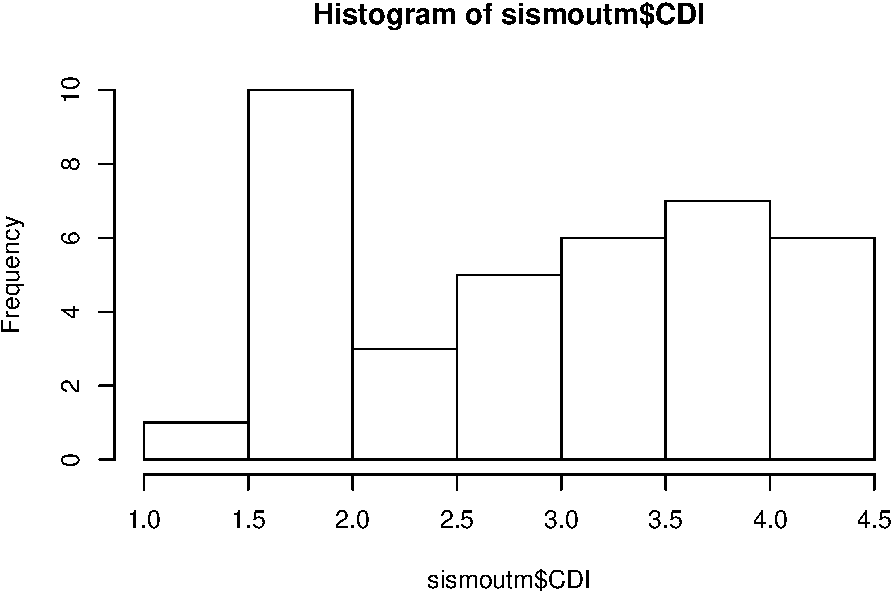
\includegraphics{proyecto_files/figure-latex/unnamed-chunk-22-1.pdf}

\begin{Shaded}
\begin{Highlighting}[]
\KeywordTok{hist}\NormalTok{(}\KeywordTok{log}\NormalTok{(sismoutm}\OperatorTok{$}\NormalTok{CDI))}
\end{Highlighting}
\end{Shaded}

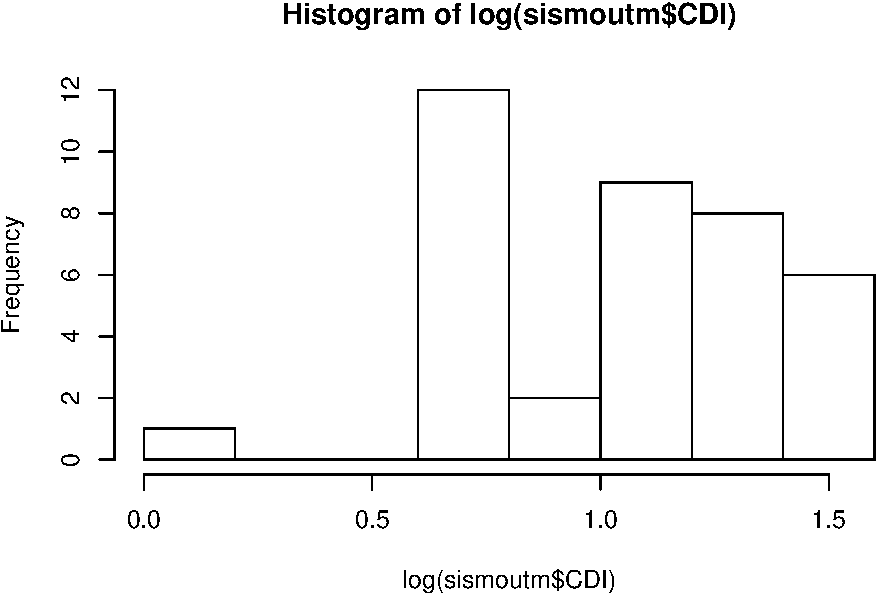
\includegraphics{proyecto_files/figure-latex/unnamed-chunk-22-2.pdf}

\begin{Shaded}
\begin{Highlighting}[]
\KeywordTok{shapiro.test}\NormalTok{(sismoutm}\OperatorTok{$}\NormalTok{CDI)}
\end{Highlighting}
\end{Shaded}

\begin{verbatim}
## 
##  Shapiro-Wilk normality test
## 
## data:  sismoutm$CDI
## W = 0.92695, p-value = 0.0161
\end{verbatim}

\begin{Shaded}
\begin{Highlighting}[]
\KeywordTok{shapiro.test}\NormalTok{(}\KeywordTok{log}\NormalTok{(sismoutm}\OperatorTok{$}\NormalTok{CDI))}
\end{Highlighting}
\end{Shaded}

\begin{verbatim}
## 
##  Shapiro-Wilk normality test
## 
## data:  log(sismoutm$CDI)
## W = 0.89265, p-value = 0.001591
\end{verbatim}

\begin{Shaded}
\begin{Highlighting}[]
\KeywordTok{qqnorm}\NormalTok{(sismoutm}\OperatorTok{$}\NormalTok{CDI)}
\end{Highlighting}
\end{Shaded}

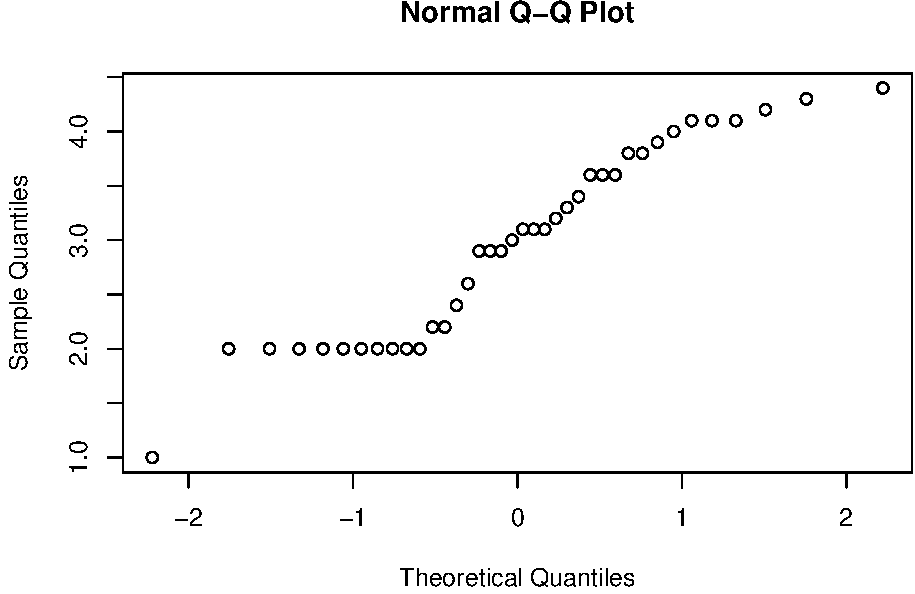
\includegraphics{proyecto_files/figure-latex/unnamed-chunk-22-3.pdf}

\begin{Shaded}
\begin{Highlighting}[]
\KeywordTok{qqnorm}\NormalTok{(}\KeywordTok{log}\NormalTok{(sismoutm}\OperatorTok{$}\NormalTok{CDI))}
\end{Highlighting}
\end{Shaded}

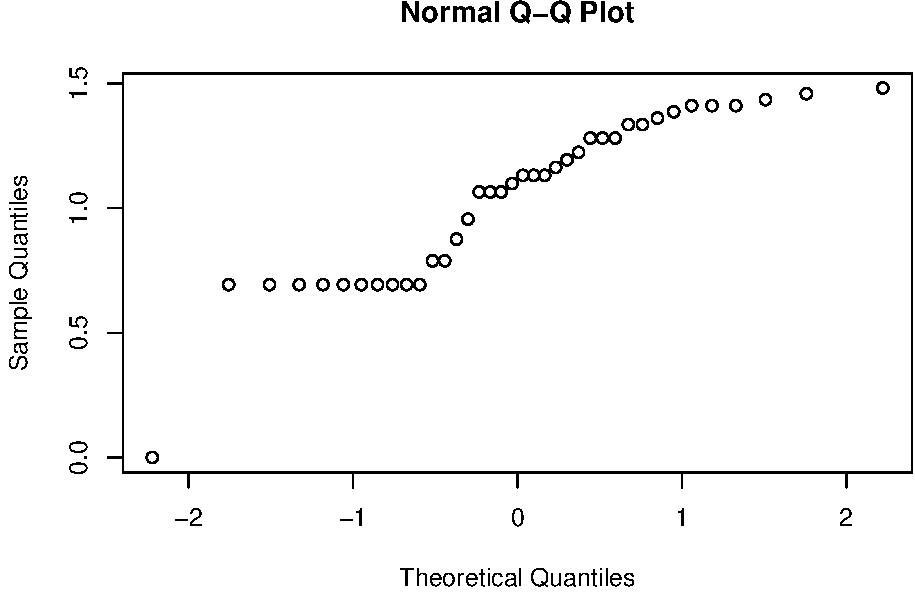
\includegraphics{proyecto_files/figure-latex/unnamed-chunk-22-4.pdf}

\begin{Shaded}
\begin{Highlighting}[]
\KeywordTok{boxplot}\NormalTok{(sismoutm}\OperatorTok{$}\NormalTok{CDI)}
\end{Highlighting}
\end{Shaded}

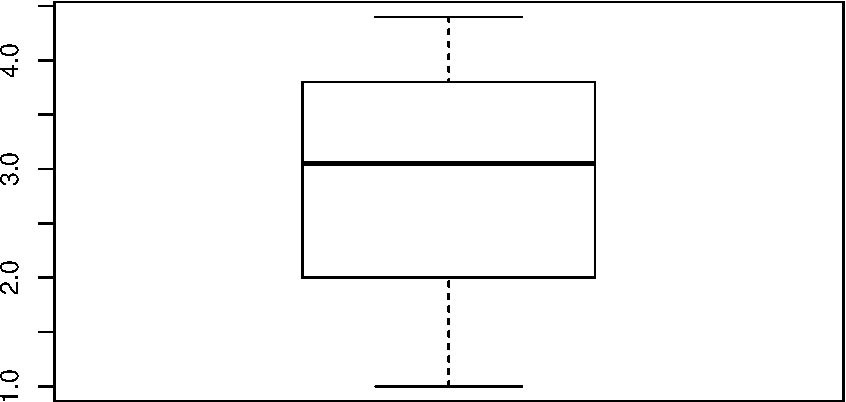
\includegraphics{proyecto_files/figure-latex/unnamed-chunk-22-5.pdf}

\subsubsection{Creacion de columna con la variable intensidad
logaritmica}\label{creacion-de-columna-con-la-variable-intensidad-logaritmica}

\begin{Shaded}
\begin{Highlighting}[]
\NormalTok{sismo <-}\StringTok{ }\NormalTok{sismoutm[,}\KeywordTok{c}\NormalTok{(}\StringTok{'F__Columns'}\NormalTok{, }\StringTok{'CDI'}\NormalTok{)]}
\NormalTok{sismo}\OperatorTok{$}\NormalTok{CDIlog <-}\StringTok{ }\KeywordTok{log}\NormalTok{(sismo}\OperatorTok{$}\NormalTok{CDI)}
\NormalTok{sismo}
\end{Highlighting}
\end{Shaded}

\begin{verbatim}
## Simple feature collection with 38 features and 3 fields
## geometry type:  POINT
## dimension:      XY
## bbox:           xmin: 222818.9 ymin: 2018261 xmax: 534804.6 ymax: 2190245
## epsg (SRID):    32619
## proj4string:    +proj=utm +zone=19 +datum=WGS84 +units=m +no_defs
## First 10 features:
##                                              F__Columns CDI
## 1                  Pimentel::Duarte::Dominican Republic 3.3
## 2  San Francisco de Macorís::Duarte::Dominican Republic 2.0
## 3              El Llano::Elías Piña::Dominican Republic 2.6
## 4         Jamao al Norte::Espaillat::Dominican Republic 2.0
## 5                   Moca::Espaillat::Dominican Republic 2.0
## 6            Hato Mayor::Hato Mayor::Dominican Republic 4.2
## 7             Higüey::La Altagracia::Dominican Republic 3.1
## 8         Otra Banda::La Altagracia::Dominican Republic 3.0
## 9              La Romana::La Romana::Dominican Republic 2.0
## 10                 La Vega::La Vega::Dominican Republic 3.4
##                    geometry    CDIlog
## 1    POINT (383293 2121116) 1.1939225
## 2    POINT (368667 2134496) 0.6931472
## 3  POINT (222818.9 2082964) 0.9555114
## 4  POINT (347977.4 2173398) 0.6931472
## 5  POINT (339341.4 2145800) 0.6931472
## 6  POINT (472597.6 2075399) 1.4350845
## 7  POINT (530591.2 2058807) 1.1314021
## 8  POINT (534804.6 2062134) 1.0986123
## 9  POINT (503168.1 2037760) 0.6931472
## 10 POINT (339165.4 2125877) 1.2237754
\end{verbatim}

\subsubsection{Representación de reportes de
intensidad}\label{representaciuxf3n-de-reportes-de-intensidad}

En la siguiente sentencia se reprecentarán gráficamente tanto la
variable original como la variable logaritmica.

\begin{Shaded}
\begin{Highlighting}[]
\KeywordTok{library}\NormalTok{(ggplot2)}
\KeywordTok{ggplot}\NormalTok{() }\OperatorTok{+}
\StringTok{  }\KeywordTok{geom_sf}\NormalTok{(}\DataTypeTok{data =}\NormalTok{ prov, }\DataTypeTok{fill =} \StringTok{'white'}\NormalTok{) }\OperatorTok{+}
\StringTok{  }\KeywordTok{geom_sf}\NormalTok{(}\DataTypeTok{data =}\NormalTok{ sismoutm, }\KeywordTok{aes}\NormalTok{(}\DataTypeTok{col =}\NormalTok{ CDI), }\DataTypeTok{size =} \DecValTok{6}\NormalTok{) }\OperatorTok{+}
\StringTok{  }\KeywordTok{scale_colour_gradient}\NormalTok{(}\DataTypeTok{low=}\StringTok{"#deebf7"}\NormalTok{, }\DataTypeTok{high=}\StringTok{"#3182bd"}\NormalTok{) }\OperatorTok{+}
\StringTok{  }\KeywordTok{geom_sf_text}\NormalTok{(}\DataTypeTok{data =}\NormalTok{ prov, }\KeywordTok{aes}\NormalTok{(}\DataTypeTok{label=}\NormalTok{TOPONIMIA), }\DataTypeTok{check_overlap =}\NormalTok{ T, }\DataTypeTok{size =} \DecValTok{2}\NormalTok{) }\OperatorTok{+}
\StringTok{  }\KeywordTok{geom_sf_text}\NormalTok{(}\DataTypeTok{data =}\NormalTok{ sismoutm, }\KeywordTok{aes}\NormalTok{(}\DataTypeTok{label=}\NormalTok{F__Columns), }\DataTypeTok{check_overlap =}\NormalTok{ T, }\DataTypeTok{size =} \FloatTok{1.5}\NormalTok{) }\OperatorTok{+}
\StringTok{  }\KeywordTok{theme_bw}\NormalTok{()}
\end{Highlighting}
\end{Shaded}

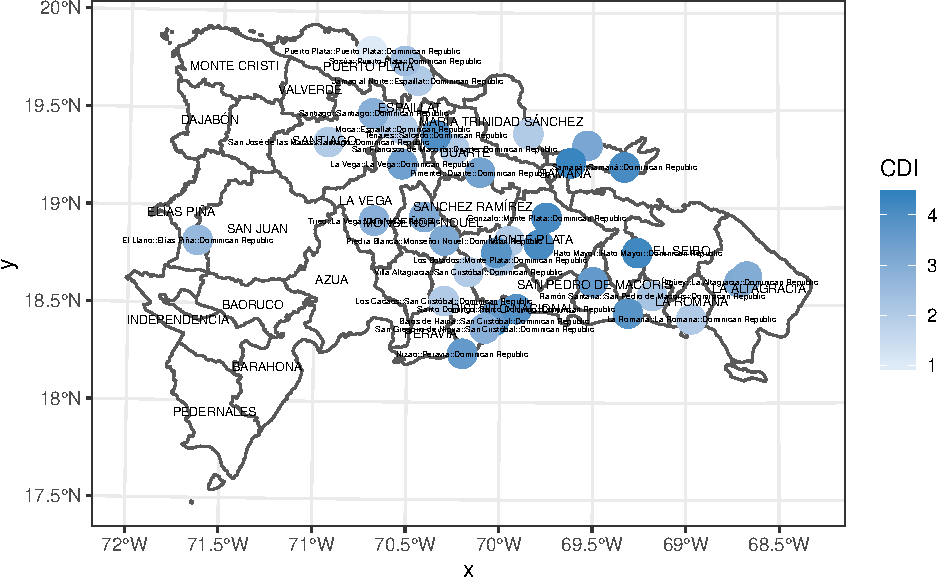
\includegraphics{proyecto_files/figure-latex/unnamed-chunk-24-1.pdf}

\begin{Shaded}
\begin{Highlighting}[]
\KeywordTok{ggplot}\NormalTok{() }\OperatorTok{+}
\StringTok{  }\KeywordTok{geom_sf}\NormalTok{(}\DataTypeTok{data =}\NormalTok{ prov, }\DataTypeTok{fill =} \StringTok{'white'}\NormalTok{) }\OperatorTok{+}
\StringTok{  }\KeywordTok{geom_sf}\NormalTok{(}\DataTypeTok{data =}\NormalTok{ sismo, }\KeywordTok{aes}\NormalTok{(}\DataTypeTok{col =}\NormalTok{ CDIlog), }\DataTypeTok{size =} \DecValTok{6}\NormalTok{) }\OperatorTok{+}
\StringTok{  }\KeywordTok{scale_colour_gradient}\NormalTok{(}\DataTypeTok{low=}\StringTok{"#deebf7"}\NormalTok{, }\DataTypeTok{high=}\StringTok{"#3182bd"}\NormalTok{) }\OperatorTok{+}
\StringTok{  }\KeywordTok{geom_sf_text}\NormalTok{(}\DataTypeTok{data =}\NormalTok{ prov, }\KeywordTok{aes}\NormalTok{(}\DataTypeTok{label=}\NormalTok{TOPONIMIA), }\DataTypeTok{check_overlap =}\NormalTok{ T, }\DataTypeTok{size =} \DecValTok{2}\NormalTok{) }\OperatorTok{+}
\StringTok{  }\KeywordTok{geom_sf_text}\NormalTok{(}\DataTypeTok{data =}\NormalTok{ sismo, }\KeywordTok{aes}\NormalTok{(}\DataTypeTok{label=}\NormalTok{F__Columns), }\DataTypeTok{check_overlap =}\NormalTok{ T, }\DataTypeTok{size =} \FloatTok{1.5}\NormalTok{) }\OperatorTok{+}
\StringTok{  }\KeywordTok{theme_bw}\NormalTok{()}
\end{Highlighting}
\end{Shaded}

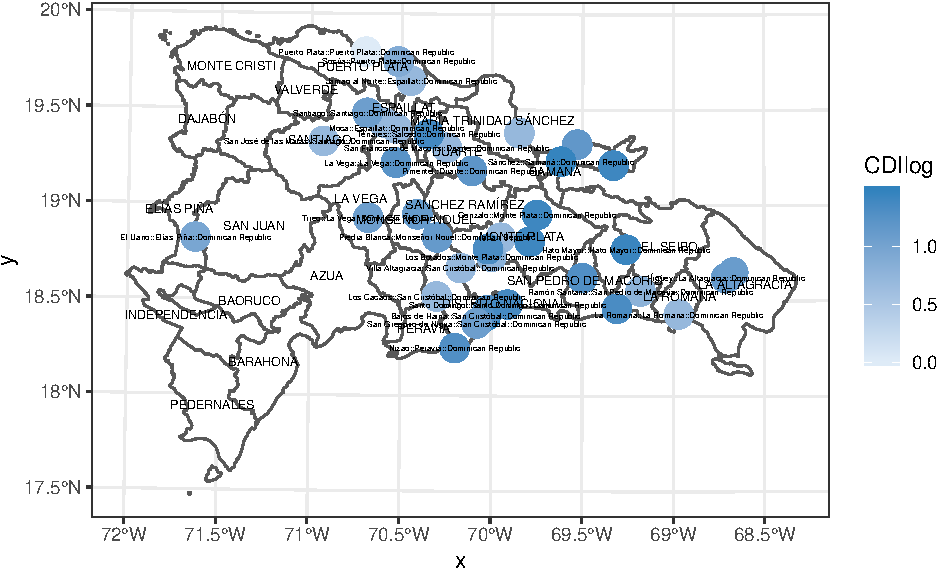
\includegraphics{proyecto_files/figure-latex/unnamed-chunk-24-2.pdf}

\subsection{3 Variograma muestral}\label{variograma-muestral}

Generacion de variogramas muestral para la intensidad del evento

\begin{Shaded}
\begin{Highlighting}[]
\NormalTok{vsismo <-}\StringTok{ }\KeywordTok{variogram}\NormalTok{(CDI}\OperatorTok{~}\DecValTok{1}\NormalTok{, sismo[}\OperatorTok{-}\DecValTok{3}\NormalTok{,])}
\NormalTok{vsismo}
\end{Highlighting}
\end{Shaded}

\begin{verbatim}
##    np      dist     gamma dir.hor dir.ver   id
## 1   3  4584.981 0.5350000       0       0 var1
## 2   7 10025.756 0.4942857       0       0 var1
## 3  13 16753.915 0.8142308       0       0 var1
## 4  15 23283.776 0.7913333       0       0 var1
## 5  25 29909.915 0.7958000       0       0 var1
## 6  31 35425.649 0.6551613       0       0 var1
## 7  23 41942.032 0.5152174       0       0 var1
## 8  31 48821.493 0.6208065       0       0 var1
## 9  28 55407.033 0.7028571       0       0 var1
## 10 30 61686.614 0.6780000       0       0 var1
## 11 33 68435.921 0.6640909       0       0 var1
## 12 35 74945.859 0.8378571       0       0 var1
## 13 25 81247.759 0.4554000       0       0 var1
## 14 35 88059.213 0.5458571       0       0 var1
## 15 33 94748.773 1.1243939       0       0 var1
\end{verbatim}

\begin{Shaded}
\begin{Highlighting}[]
\KeywordTok{plot}\NormalTok{(vsismo, }\DataTypeTok{plot.numbers =}\NormalTok{ T)}
\end{Highlighting}
\end{Shaded}

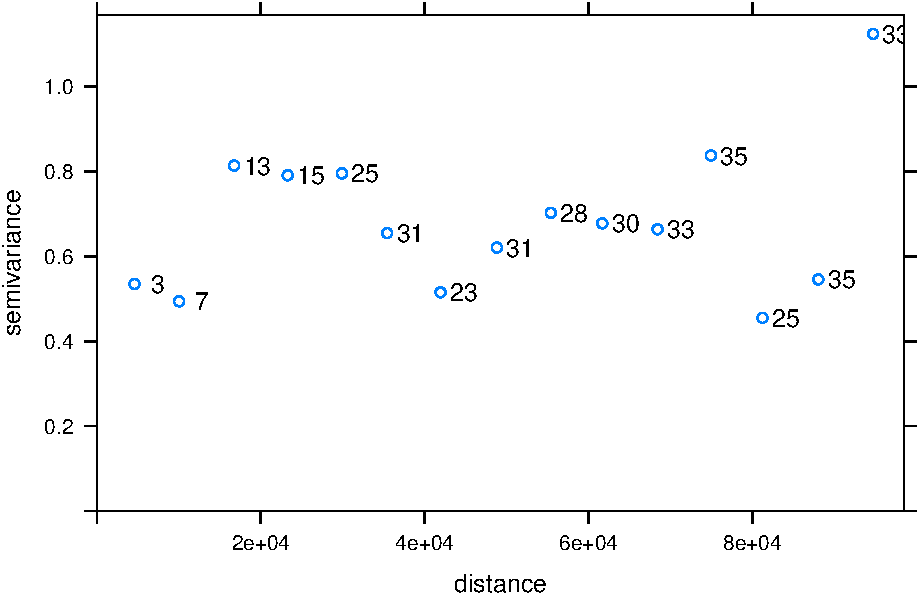
\includegraphics{proyecto_files/figure-latex/unnamed-chunk-25-1.pdf}

\begin{Shaded}
\begin{Highlighting}[]
\NormalTok{vsismolog <-}\StringTok{ }\KeywordTok{variogram}\NormalTok{(CDIlog}\OperatorTok{~}\DecValTok{1}\NormalTok{, sismo[}\OperatorTok{-}\DecValTok{3}\NormalTok{,])}
\NormalTok{vsismolog}
\end{Highlighting}
\end{Shaded}

\begin{verbatim}
##    np      dist      gamma dir.hor dir.ver   id
## 1   3  4584.981 0.05667565       0       0 var1
## 2   7 10025.756 0.05614854       0       0 var1
## 3  13 16753.915 0.09676437       0       0 var1
## 4  15 23283.776 0.11080402       0       0 var1
## 5  25 29909.915 0.10352200       0       0 var1
## 6  31 35425.649 0.09174189       0       0 var1
## 7  23 41942.032 0.07554403       0       0 var1
## 8  31 48821.493 0.08167166       0       0 var1
## 9  28 55407.033 0.09162158       0       0 var1
## 10 30 61686.614 0.09356106       0       0 var1
## 11 33 68435.921 0.08764143       0       0 var1
## 12 35 74945.859 0.10718693       0       0 var1
## 13 25 81247.759 0.05175244       0       0 var1
## 14 35 88059.213 0.05987754       0       0 var1
## 15 33 94748.773 0.15344586       0       0 var1
\end{verbatim}

\begin{Shaded}
\begin{Highlighting}[]
\KeywordTok{plot}\NormalTok{(vsismolog, }\DataTypeTok{plot.numbers =}\NormalTok{ T)}
\end{Highlighting}
\end{Shaded}

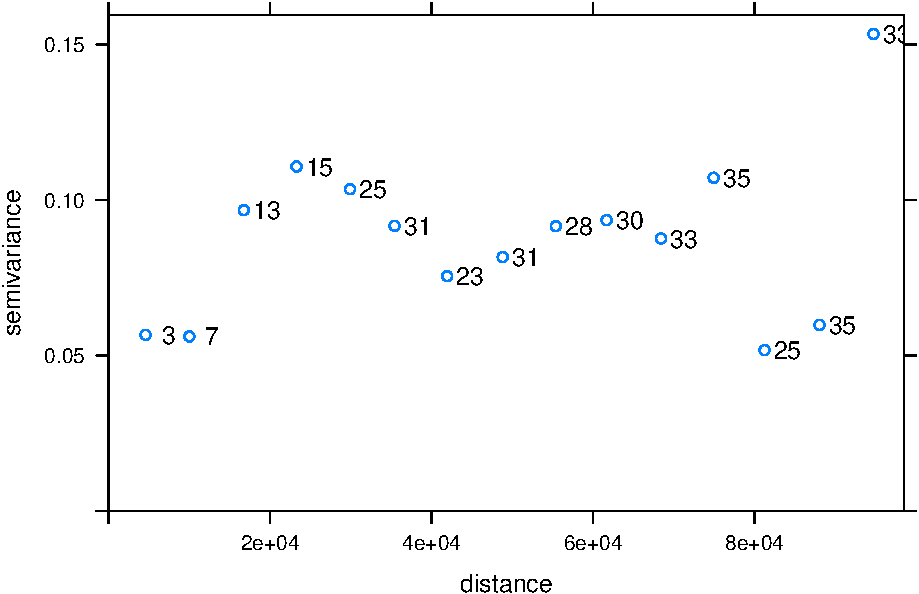
\includegraphics{proyecto_files/figure-latex/unnamed-chunk-25-2.pdf}

\begin{Shaded}
\begin{Highlighting}[]
\NormalTok{vsismolog <-}\StringTok{ }\KeywordTok{variogram}\NormalTok{(CDIlog}\OperatorTok{~}\DecValTok{1}\NormalTok{, sismo[}\OperatorTok{-}\DecValTok{3}\NormalTok{,], }\DataTypeTok{alpha =} \DecValTok{0}\NormalTok{, }\DataTypeTok{tol.hor =} \DecValTok{90}\OperatorTok{/}\DecValTok{4}\NormalTok{)}
\NormalTok{vsismolog}
\end{Highlighting}
\end{Shaded}

\begin{verbatim}
##    np      dist      gamma dir.hor dir.ver   id
## 1   1  3483.671 0.02013436       0       0 var1
## 2   1 16054.490 0.00000000       0       0 var1
## 3   3 23355.594 0.16354323       0       0 var1
## 4   5 30671.385 0.09243373       0       0 var1
## 5  13 35856.397 0.11441264       0       0 var1
## 6   4 42058.159 0.12191487       0       0 var1
## 7  14 48475.921 0.11713332       0       0 var1
## 8   7 55430.965 0.08257598       0       0 var1
## 9   8 61727.363 0.07117756       0       0 var1
## 10  7 68425.528 0.15423133       0       0 var1
## 11  5 75840.950 0.08533433       0       0 var1
## 12  8 81742.497 0.06540322       0       0 var1
## 13  4 88201.455 0.01146635       0       0 var1
## 14  7 94415.997 0.18919368       0       0 var1
\end{verbatim}

\begin{Shaded}
\begin{Highlighting}[]
\KeywordTok{plot}\NormalTok{(vsismolog, }\DataTypeTok{plot.numbers =}\NormalTok{ T)}
\end{Highlighting}
\end{Shaded}

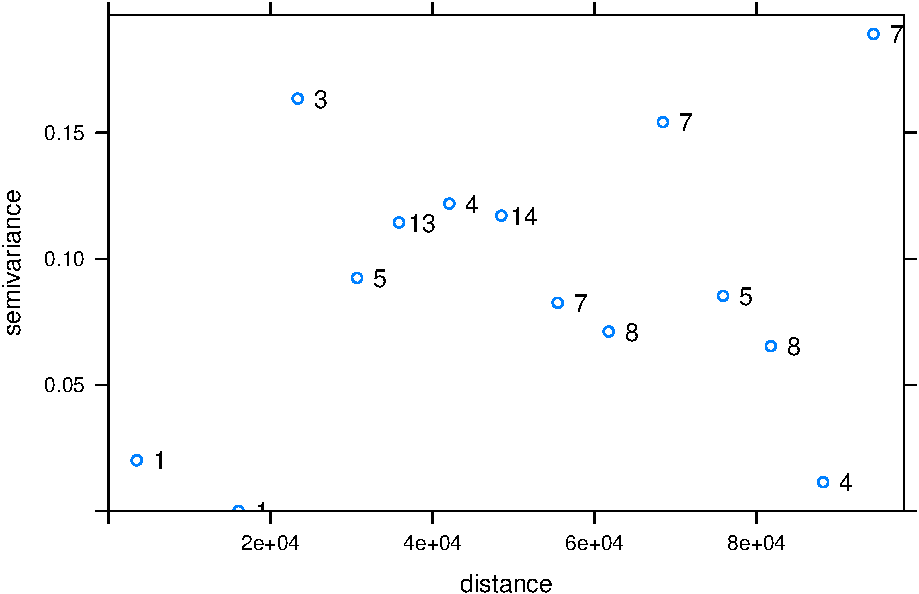
\includegraphics{proyecto_files/figure-latex/unnamed-chunk-25-3.pdf}

\subsection{3 Variogramas modelo}\label{variogramas-modelo}

\begin{Shaded}
\begin{Highlighting}[]
\NormalTok{vsismo_m <-}\StringTok{ }\KeywordTok{fit.variogram}\NormalTok{(vsismo, }\KeywordTok{vgm}\NormalTok{(}\DataTypeTok{model =} \StringTok{"Sph"}\NormalTok{, }\DataTypeTok{range =} \DecValTok{20000}\NormalTok{))}
\NormalTok{vsismo_m}
\end{Highlighting}
\end{Shaded}

\begin{verbatim}
##   model     psill    range
## 1   Sph 0.6698106 7552.753
\end{verbatim}

\begin{Shaded}
\begin{Highlighting}[]
\KeywordTok{plot}\NormalTok{(vsismo, vsismo_m, }\DataTypeTok{plot.numbers =}\NormalTok{ T)}
\end{Highlighting}
\end{Shaded}

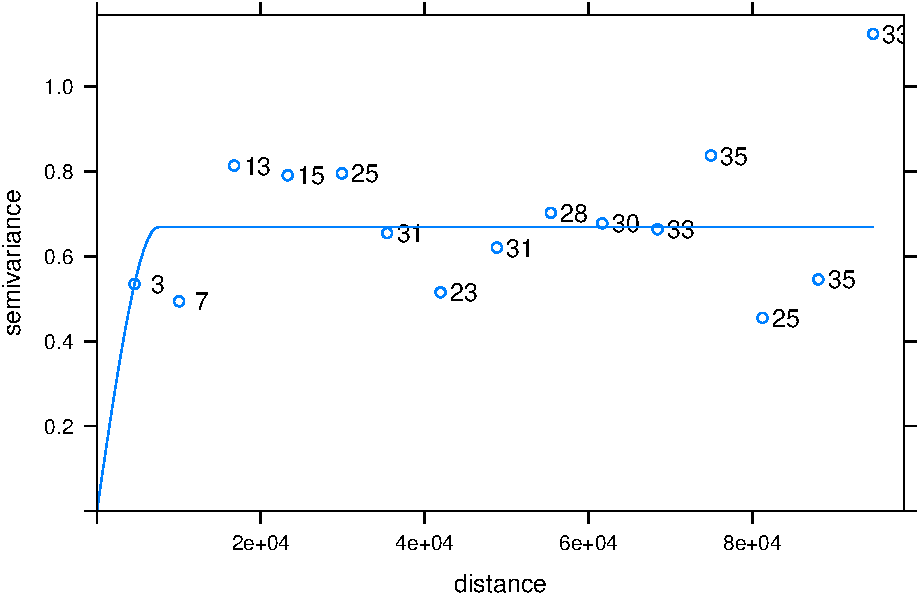
\includegraphics{proyecto_files/figure-latex/unnamed-chunk-26-1.pdf}

\begin{Shaded}
\begin{Highlighting}[]
\NormalTok{vsismolog_m <-}\StringTok{ }\KeywordTok{fit.variogram}\NormalTok{(vsismolog, }\KeywordTok{vgm}\NormalTok{(}\DataTypeTok{model =} \StringTok{"Wav"}\NormalTok{, }\DataTypeTok{range =} \DecValTok{15000}\NormalTok{))}
\end{Highlighting}
\end{Shaded}

\begin{verbatim}
## Warning in fit.variogram(vsismolog, vgm(model = "Wav", range = 15000)): No
## convergence after 200 iterations: try different initial values?
\end{verbatim}

\begin{Shaded}
\begin{Highlighting}[]
\NormalTok{vsismolog_m}
\end{Highlighting}
\end{Shaded}

\begin{verbatim}
##   model     psill range
## 1   Wav 0.1048178 15000
\end{verbatim}

\begin{Shaded}
\begin{Highlighting}[]
\KeywordTok{plot}\NormalTok{(vsismolog, vsismolog_m, }\DataTypeTok{plot.numbers =}\NormalTok{ T)}
\end{Highlighting}
\end{Shaded}

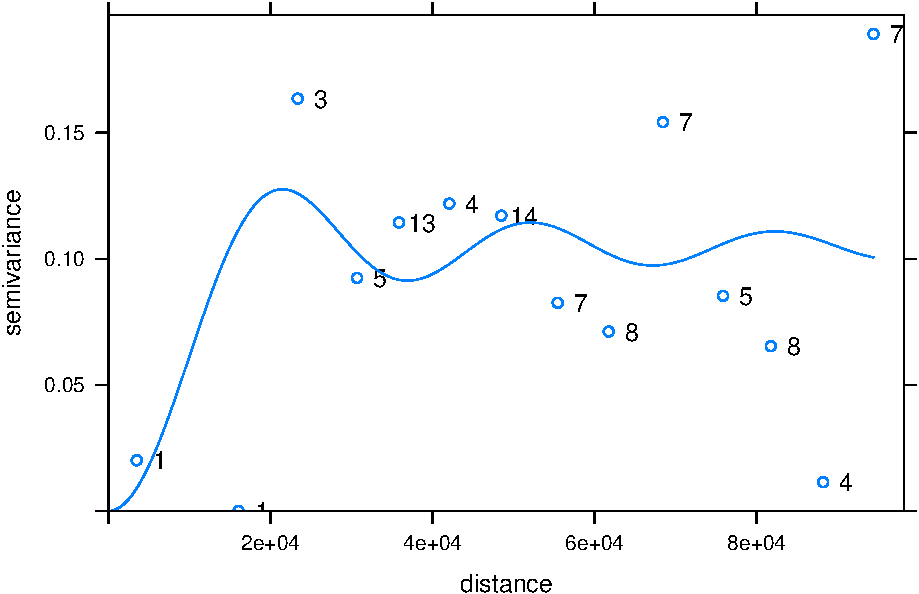
\includegraphics{proyecto_files/figure-latex/unnamed-chunk-26-2.pdf}

\begin{Shaded}
\begin{Highlighting}[]
\NormalTok{vsismolog_m <-}\StringTok{ }\KeywordTok{fit.variogram}\NormalTok{(vsismolog, }\KeywordTok{vgm}\NormalTok{(}\DataTypeTok{model =} \StringTok{"Exp"}\NormalTok{, }\DataTypeTok{range =} \DecValTok{30000}\NormalTok{))}
\NormalTok{vsismolog_m}
\end{Highlighting}
\end{Shaded}

\begin{verbatim}
##   model     psill    range
## 1   Exp 0.1179361 16212.96
\end{verbatim}

\begin{Shaded}
\begin{Highlighting}[]
\KeywordTok{plot}\NormalTok{(vsismolog, vsismolog_m, }\DataTypeTok{plot.numbers =}\NormalTok{ T)}
\end{Highlighting}
\end{Shaded}

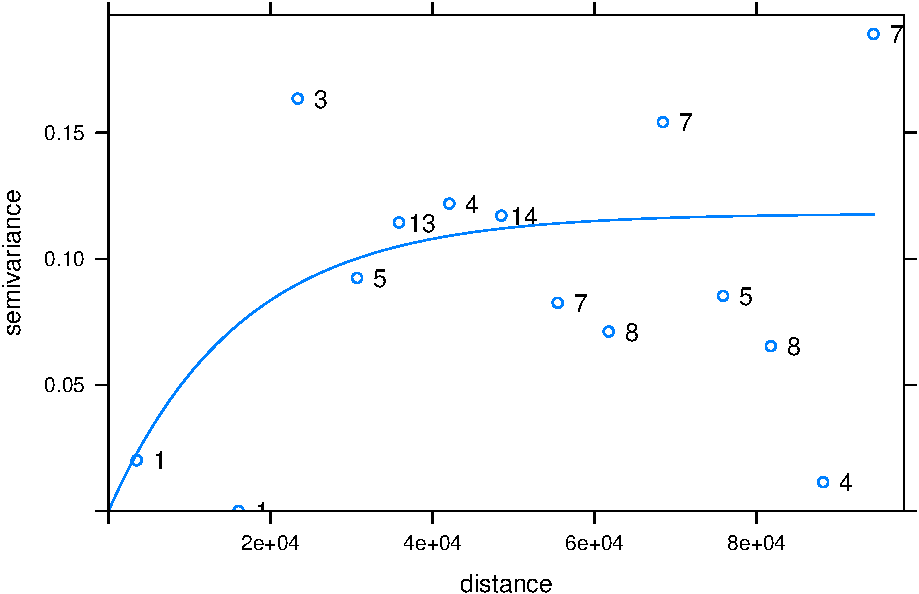
\includegraphics{proyecto_files/figure-latex/unnamed-chunk-26-3.pdf}

\subsubsection{Interpolación por kriging
ordinario}\label{interpolaciuxf3n-por-kriging-ordinario-1}

Antes de realizar la interpolación, necesitamos una cuadrícula que
``llenaremos'' con las predicciones. Creemos una cuadrícula para RD, de
resolución, 1x1km.

\begin{Shaded}
\begin{Highlighting}[]
\KeywordTok{library}\NormalTok{(stars)}
\end{Highlighting}
\end{Shaded}

\begin{verbatim}
## Loading required package: abind
\end{verbatim}

\begin{Shaded}
\begin{Highlighting}[]
\NormalTok{grd <-}\StringTok{ }\KeywordTok{st_bbox}\NormalTok{(prov) }\OperatorTok
\StringTok{  }\KeywordTok{st_as_stars}\NormalTok{(}\DataTypeTok{dx =} \DecValTok{1000}\NormalTok{) }\OperatorTok\StringTok{ }\CommentTok{#100 metros=1km de resolución espacial}
\StringTok{  }\KeywordTok{st_set_crs}\NormalTok{(crswgs84utm) }\OperatorTok
\StringTok{  }\KeywordTok{st_crop}\NormalTok{(prov)}
\NormalTok{grd}
\end{Highlighting}
\end{Shaded}

\begin{verbatim}
## stars object with 2 dimensions and 1 attribute
## attribute(s):
##     values      
##  Min.   :0      
##  1st Qu.:0      
##  Median :0      
##  Mean   :0      
##  3rd Qu.:0      
##  Max.   :0      
##  NA's   :58017  
## dimension(s):
##   from  to  offset delta                       refsys point values    
## x    1 390  182216  1000 +proj=utm +zone=19 +datum...    NA   NULL [x]
## y    1 272 2205216 -1000 +proj=utm +zone=19 +datum...    NA   NULL [y]
\end{verbatim}

\begin{Shaded}
\begin{Highlighting}[]
\KeywordTok{plot}\NormalTok{(grd)}
\end{Highlighting}
\end{Shaded}

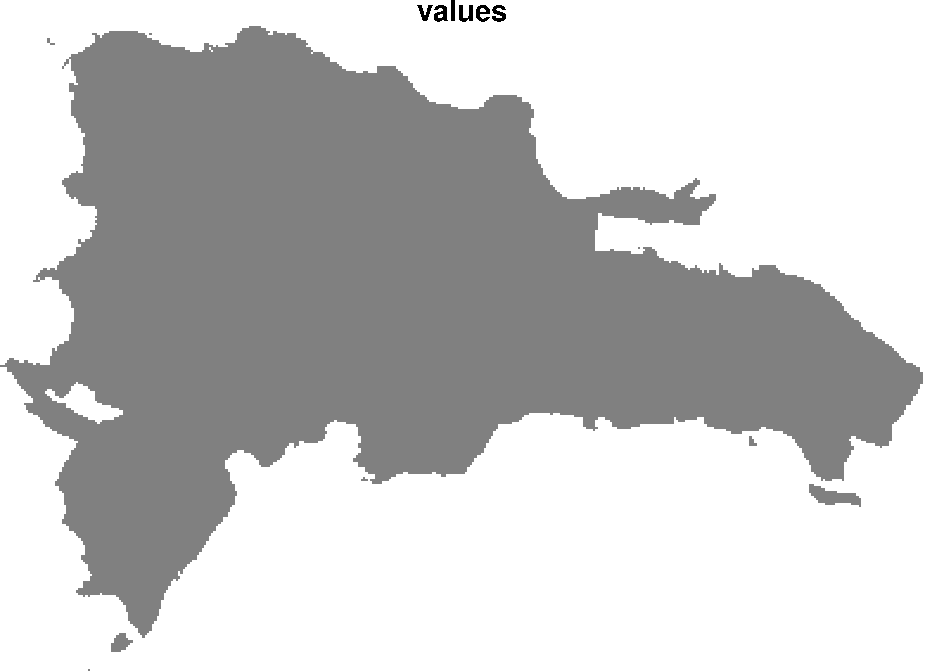
\includegraphics{proyecto_files/figure-latex/unnamed-chunk-27-1.pdf}

Interpolación de los datos

\begin{Shaded}
\begin{Highlighting}[]
\NormalTok{ik <-}\StringTok{ }\KeywordTok{krige}\NormalTok{(}\DataTypeTok{formula =}\NormalTok{ CDIlog}\OperatorTok{~}\DecValTok{1}\NormalTok{, }\DataTypeTok{locations =}\NormalTok{ sismo, }\DataTypeTok{newdata =}\NormalTok{ grd, }\DataTypeTok{model =}\NormalTok{ vsismolog_m)}
\end{Highlighting}
\end{Shaded}

\begin{verbatim}
## [using ordinary kriging]
\end{verbatim}

\begin{Shaded}
\begin{Highlighting}[]
\NormalTok{ik}
\end{Highlighting}
\end{Shaded}

\begin{verbatim}
## stars object with 2 dimensions and 2 attributes
## attribute(s):
##    var1.pred       var1.var     
##  Min.   :0.04    Min.   :0.00   
##  1st Qu.:0.98    1st Qu.:0.08   
##  Median :1.02    Median :0.11   
##  Mean   :1.02    Mean   :0.10   
##  3rd Qu.:1.06    3rd Qu.:0.12   
##  Max.   :1.46    Max.   :0.12   
##  NA's   :58017   NA's   :58017  
## dimension(s):
##   from  to  offset delta                       refsys point values    
## x    1 390  182216  1000 +proj=utm +zone=19 +datum...    NA   NULL [x]
## y    1 272 2205216 -1000 +proj=utm +zone=19 +datum...    NA   NULL [y]
\end{verbatim}

\begin{Shaded}
\begin{Highlighting}[]
\KeywordTok{summary}\NormalTok{(}\KeywordTok{as.vector}\NormalTok{(}\KeywordTok{exp}\NormalTok{(ik}\OperatorTok{$}\NormalTok{var1.pred))) }
\end{Highlighting}
\end{Shaded}

\begin{verbatim}
##    Min. 1st Qu.  Median    Mean 3rd Qu.    Max.    NA's 
##    1.04    2.67    2.77    2.80    2.88    4.31   58017
\end{verbatim}

\begin{Shaded}
\begin{Highlighting}[]
\KeywordTok{plot}\NormalTok{(ik)}
\end{Highlighting}
\end{Shaded}

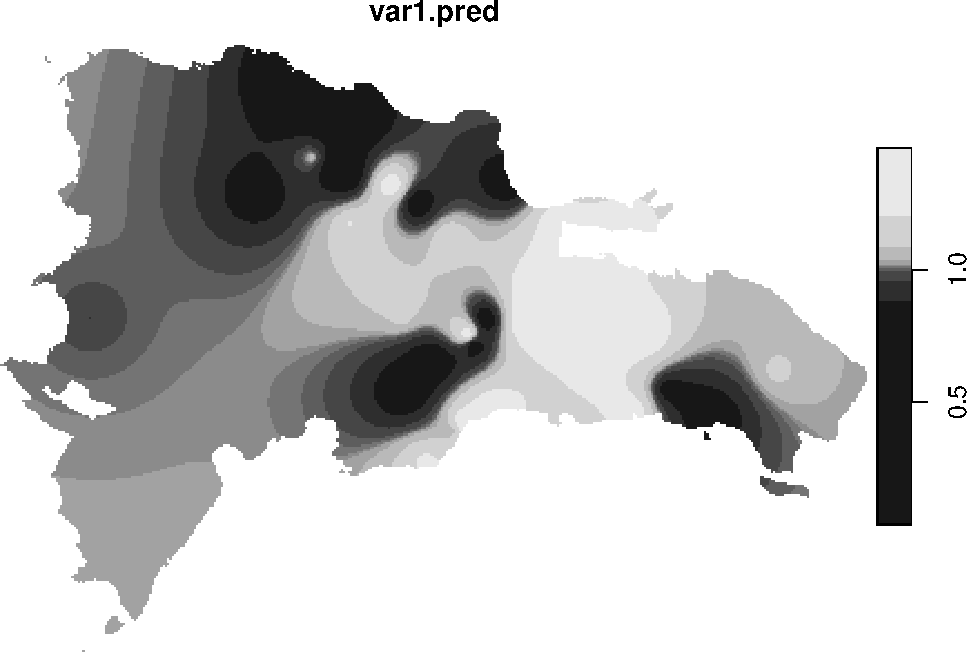
\includegraphics{proyecto_files/figure-latex/unnamed-chunk-28-1.pdf}

Utilicemos ggplot para representar el objeto resultante

\begin{Shaded}
\begin{Highlighting}[]
\KeywordTok{ggplot}\NormalTok{() }\OperatorTok{+}
\StringTok{  }\KeywordTok{geom_stars}\NormalTok{(}\DataTypeTok{data =}\NormalTok{ ik, }\KeywordTok{aes}\NormalTok{(}\DataTypeTok{fill =} \KeywordTok{exp}\NormalTok{(var1.pred), }\DataTypeTok{x =}\NormalTok{ x, }\DataTypeTok{y =}\NormalTok{ y)) }\OperatorTok{+}\StringTok{ }
\StringTok{  }\KeywordTok{scale_fill_gradientn}\NormalTok{(}\DataTypeTok{colours =} \KeywordTok{brewer.pal}\NormalTok{(}\DecValTok{9}\NormalTok{, }\StringTok{'YlOrBr'}\NormalTok{)) }\OperatorTok{+}
\StringTok{  }\KeywordTok{geom_sf}\NormalTok{(}\DataTypeTok{data =} \KeywordTok{st_cast}\NormalTok{(prov, }\StringTok{"MULTILINESTRING"}\NormalTok{)) }\OperatorTok{+}
\StringTok{  }\KeywordTok{geom_sf}\NormalTok{(}\DataTypeTok{data =}\NormalTok{ sismo) }\OperatorTok{+}
\StringTok{  }\KeywordTok{geom_sf_text}\NormalTok{(}\DataTypeTok{data =}\NormalTok{ sismo, }\KeywordTok{aes}\NormalTok{(}\DataTypeTok{label=}\KeywordTok{round}\NormalTok{(}\KeywordTok{exp}\NormalTok{(CDIlog),}\DecValTok{0}\NormalTok{)), }\DataTypeTok{col =} \StringTok{'white'}\NormalTok{, }\DataTypeTok{check_overlap =}\NormalTok{ T, }\DataTypeTok{size =} \DecValTok{4}\NormalTok{, }\DataTypeTok{nudge_x =} \DecValTok{5000}\NormalTok{) }\OperatorTok{+}
\StringTok{  }\KeywordTok{theme_bw}\NormalTok{()}
\end{Highlighting}
\end{Shaded}

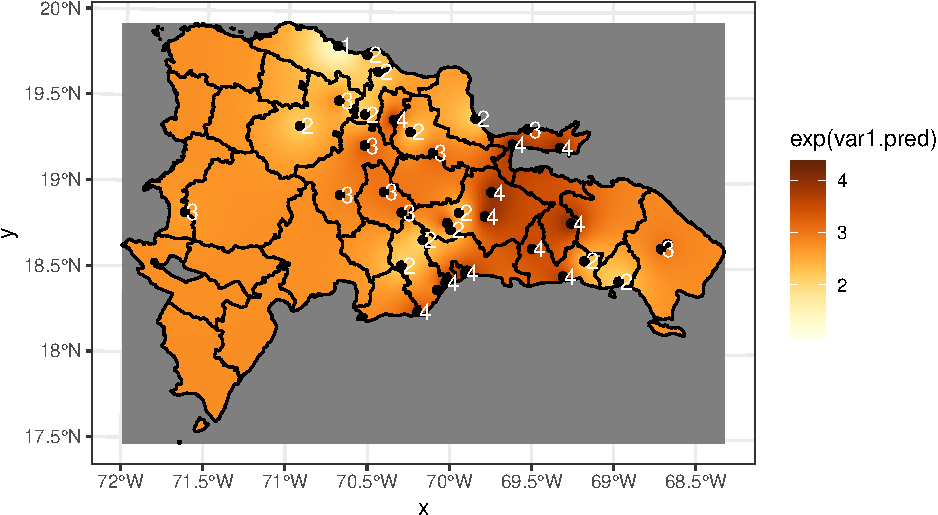
\includegraphics{proyecto_files/figure-latex/unnamed-chunk-29-1.pdf}

\section{Referencias}\label{referencias}

{[}1{]}-Material de Apoyo de la asignatura Analisis Espacial de la
Maestria en Teledeteccion y Ciencias Gegraficas de Escuela de Ciencias
Geofrafica de la Universidad Autonoma de Santo Domingo, impartida por el
Maestro José Ramon Martinez Beltra.

{[}2{]}-
\url{https://earthquake.usgs.gov/earthquakes/eventpage/us1000ehsg/dyfi/intensity}




\newpage
\singlespacing 
\end{document}
